% ============================================================================
% Supplementary Material for FL-EHDS (FLICS 2026)
% ============================================================================
\documentclass[conference]{IEEEtran}

\usepackage{cite}
\usepackage{amsmath,amssymb,amsfonts}
\usepackage{graphicx}
\usepackage{textcomp}
\usepackage{xcolor}
\usepackage{booktabs}
\usepackage{hyperref}
\usepackage{url}
\usepackage{tikz}
\usetikzlibrary{shapes.geometric, arrows.meta, positioning, fit, backgrounds, calc}
\usepackage{pgfplots}
\pgfplotsset{compat=1.18}

\begin{document}

\title{Supplementary Material:\\FL-EHDS: A Privacy-Preserving Federated Learning Framework for the European Health Data Space}

\author{
    \IEEEauthorblockN{Fabio Liberti}
    \IEEEauthorblockA{
        Department of Computer Science\\
        Universitas Mercatorum, Rome, Italy\\
        fabio.liberti@unimercatorum.it\\
        ORCID: 0000-0003-3019-5411
    }
}

\maketitle

\begin{abstract}
This document provides supplementary material for the FL-EHDS paper, including complete algorithm pseudocode for all framework components, extended experimental figures, detailed algorithm comparison analysis, advanced FL paradigm descriptions, infrastructure component specifications, extended EHDS interoperability details, and clinical imaging experiment configurations. The open-source reference implementation ($\sim$40K lines, 159 modules) is available at \url{https://github.com/FabioLiberti/FL-EHDS-FLICS2026}.
\end{abstract}

% ============================================================================
\section{PRISMA Flow Diagram}
\label{sec:prisma}
% ============================================================================

\begin{figure*}[t]
\centering
\includegraphics[width=\textwidth]{figures/fig_prisma_flowchart.pdf}
\caption{PRISMA 2020 flow diagram for the systematic review. Database searches across PubMed, IEEE Xplore, Scopus, Web of Science, and arXiv identified 847 records; after deduplication (264 removed) and screening, 47 studies met inclusion criteria (2022--2026, FL/EHDS focus, peer-reviewed or recognized institutional origin). Additional records from institutional websites (n=15), organisations (n=8), and citation searching (n=2) were assessed but did not contribute to the final inclusion set. Adapted from Page et al.\ (BMJ 2021;372:n71), licensed under CC BY 4.0.}
\label{fig:prisma}
\end{figure*}

% ============================================================================
\section{Algorithm Pseudocode}
\label{sec:pseudocode}
% ============================================================================

This section provides formal algorithmic descriptions of all FL-EHDS framework components. Each algorithm is presented with: (1)~a contextual explanation of \textit{why} the component is needed in the EHDS regulatory context; (2)~the formal pseudocode; and (3)~practical considerations for deployment. The algorithms are organized following the data flow through the three-layer architecture: governance validation (Layer~1), privacy-preserving aggregation (Layer~2), and local data processing (Layer~3).

\noindent\textbf{Reading guide:} Algorithms~S1--S4 form the core FL-EHDS training pipeline. Algorithms~S5--S6 address EHDS-specific challenges (non-IID data and citizen opt-out). Algorithms~S7--S8 handle data preprocessing and privacy budget management.

\subsection{FedAvg with EHDS Compliance}

Algorithm~S1 presents the core federated averaging procedure adapted for EHDS regulatory requirements, operating in a client-server architecture where the central aggregator coordinates training across distributed hospital nodes within a Secure Processing Environment.

\textbf{Key Design Decisions:}
\begin{itemize}
    \item \textbf{ValidatePermit}: Before each round, the HDAB-issued permit is verified against temporal bounds and Article~53 permitted purposes.
    \item \textbf{SelectParticipants}: Configurable client selection---full participation or sampling for large federations.
    \item \textbf{FilterOptedOut}: Records from citizens who exercised Article~71 opt-out rights are excluded \textit{before} gradient computation.
    \item \textbf{Weighted Aggregation}: Gradients weighted by local dataset size ($n_h$), following original FedAvg~\cite{mcmahan2017communication}.
    \item \textbf{ClipGradient}: L2-norm clipping bounds individual contributions, providing sensitivity bounds for DP.
\end{itemize}

\begin{figure}[htbp]
\centering
\fbox{\parbox{0.92\columnwidth}{
\small
\textbf{Algorithm S1: FL-EHDS FedAvg Training}\\[2pt]
\textbf{Input:} Hospitals $\mathcal{H} = \{h_1, \ldots, h_K\}$, permit $P$, rounds $T$\\
\textbf{Output:} Global model $\theta^{(T)}$\\[3pt]
\textbf{Server executes:}\\
\hspace*{4mm}Initialize $\theta^{(0)}$\\
\hspace*{4mm}\textbf{for} round $t = 1$ to $T$ \textbf{do}\\
\hspace*{8mm}\textit{// Governance check (Layer 1)}\\
\hspace*{8mm}\textbf{if} not ValidatePermit($P$, $t$) \textbf{then abort}\\
\hspace*{8mm}$\mathcal{H}_t \leftarrow$ SelectParticipants($\mathcal{H}$)\\
\hspace*{8mm}\textbf{for each} hospital $h \in \mathcal{H}_t$ \textbf{in parallel do}\\
\hspace*{12mm}$\Delta_h^{(t)}, n_h \leftarrow$ LocalTrain($h$, $\theta^{(t-1)}$)\\
\hspace*{8mm}\textit{// Aggregation with privacy (Layer 2)}\\
\hspace*{8mm}$\theta^{(t)} \leftarrow \theta^{(t-1)} + \frac{1}{\sum_h n_h} \sum_{h \in \mathcal{H}_t} n_h \cdot \Delta_h^{(t)}$\\
\hspace*{8mm}LogCompliance($t$, $\mathcal{H}_t$)\\
\hspace*{4mm}\textbf{return} $\theta^{(T)}$\\[3pt]
\textbf{LocalTrain}($h$, $\theta$) \textbf{at hospital} $h$:\\
\hspace*{4mm}\textit{// Opt-out filtering (Article 71)}\\
\hspace*{4mm}$\mathcal{D}_h \leftarrow$ FilterOptedOut($\mathcal{D}_h$, OptOutRegistry)\\
\hspace*{4mm}$\theta_h \leftarrow \theta$\\
\hspace*{4mm}\textbf{for} epoch $e = 1$ to $E$ \textbf{do}\\
\hspace*{8mm}\textbf{for} batch $\mathcal{B} \in \mathcal{D}_h$ \textbf{do}\\
\hspace*{12mm}$\theta_h \leftarrow \theta_h - \eta \nabla \mathcal{L}(\theta_h; \mathcal{B})$\\
\hspace*{4mm}$\Delta_h \leftarrow \theta_h - \theta$\\
\hspace*{4mm}\textit{// Privacy protection (Layer 3)}\\
\hspace*{4mm}$\Delta_h \leftarrow$ ClipGradient($\Delta_h$, $C$)\\
\hspace*{4mm}\textbf{return} $\Delta_h$, $|\mathcal{D}_h|$
}}
\end{figure}

\textbf{Relationship to subsequent components:} The \texttt{ClipGradient} operation in Algorithm~S1 establishes a bounded sensitivity $C$ for each client's contribution. This bound is the prerequisite for Algorithm~S2 (Gaussian DP), which calibrates noise proportional to $C$. Meanwhile, \texttt{ValidatePermit} invokes Algorithm~S3 (Permit Validation) and \texttt{FilterOptedOut} invokes Algorithm~S6 (Opt-Out Filtering).

\subsection{Gaussian Differential Privacy Mechanism}

Algorithm~S2 implements the Gaussian mechanism for differential privacy, applied at the aggregation server after receiving clipped gradients.

\textbf{Mathematical Foundation:} The noise scale $\sigma = C \cdot \sqrt{2\ln(1.25/\delta)}/\varepsilon$ guarantees $(\varepsilon, \delta)$-DP. The cumulative privacy expenditure is tracked using R\'enyi DP (RDP)~\cite{mironov2017renyi} composition, providing 5--6$\times$ tighter bounds than naive composition.

\textbf{Practical Considerations:}
\begin{itemize}
    \item $\varepsilon = 10$: moderate noise, expected accuracy drop in the 5--6pp range (consistent with Wei et al.~\cite{wei2020federated})
    \item $\varepsilon = 1$: strong privacy, larger accuracy cost; a comprehensive ablation across $\varepsilon$ values is planned
    \item The $\varepsilon$ selection must be negotiated with HDABs during permit approval
\end{itemize}

\begin{figure}[htbp]
\centering
\fbox{\parbox{0.92\columnwidth}{
\small
\textbf{Algorithm S2: Gaussian DP Mechanism}\\[2pt]
\textbf{Input:} Gradient $\Delta$, sensitivity $C$, privacy budget $\varepsilon$, $\delta$\\
\textbf{Output:} Noisy gradient $\tilde{\Delta}$\\[3pt]
\textit{// Compute noise scale from Gaussian mechanism}\\
$\sigma \leftarrow C \cdot \sqrt{2 \ln(1.25/\delta)} / \varepsilon$\\[2pt]
\textit{// Add calibrated Gaussian noise to each parameter}\\
\textbf{for each} parameter $w \in \Delta$ \textbf{do}\\
\hspace*{4mm}$\tilde{w} \leftarrow w + \mathcal{N}(0, \sigma^2)$\\[2pt]
\textit{// Track cumulative privacy expenditure}\\
PrivacyAccountant.spend($\varepsilon$)\\
\textbf{if} PrivacyAccountant.budget\_exhausted() \textbf{then}\\
\hspace*{4mm}\textbf{raise} PrivacyBudgetExhaustedError\\[2pt]
\textbf{return} $\tilde{\Delta}$
}}
\end{figure}

\textbf{Integration with privacy budget:} The $\varepsilon$ consumed by Algorithm~S2 in each round is tracked by Algorithm~S8 (RDP Privacy Budget Accountant). If the cumulative budget exceeds the threshold approved in the HDAB data permit, training is automatically terminated. The next algorithm (S3) formalizes the permit validation that authorizes each round.

\subsection{HDAB Permit Validation}

Algorithm~S3 ensures all FL operations comply with the data permit issued by HDABs. Under EHDS Article~53, secondary use of health data is only lawful for specifically enumerated purposes (scientific research, public health surveillance, AI training for health). The permit validation module is invoked at the beginning of every FL round---not just at training start---to guarantee continuous compliance even if a permit is revoked mid-study or its temporal validity expires. Each validation event is logged as a GDPR Article~30 processing record, creating an immutable audit trail that regulators can inspect.

\textbf{EHDS Governance Role:} This algorithm is the enforcement point between the Governance Layer (Layer~1) and the FL Orchestration Layer (Layer~2). Without it, a permit expiring at round~15 of a 20-round study would allow unauthorized data processing for rounds~16--20.

\begin{figure}[htbp]
\centering
\fbox{\parbox{0.92\columnwidth}{
\small
\textbf{Algorithm S3: Data Permit Validation}\\[2pt]
\textbf{Input:} Permit $P$, round $t$, requested categories $\mathcal{C}$\\
\textbf{Output:} Boolean validity\\[3pt]
\textit{// Check temporal validity}\\
\textbf{if} CurrentTime() $>$ $P$.valid\_until \textbf{then}\\
\hspace*{4mm}\textbf{raise} PermitExpiredError\\[2pt]
\textit{// Check purpose alignment (Article 53)}\\
\textbf{if} $P$.purpose $\notin$ AllowedPurposes \textbf{then}\\
\hspace*{4mm}\textbf{raise} PurposeMismatchError\\[2pt]
\textit{// Check data category authorization}\\
\textbf{for each} category $c \in \mathcal{C}$ \textbf{do}\\
\hspace*{4mm}\textbf{if} $c \notin P$.authorized\_categories \textbf{then}\\
\hspace*{8mm}\textbf{raise} UnauthorizedCategoryError\\[2pt]
\textit{// Log access for GDPR Article 30}\\
AuditTrail.log(permit=$P$, round=$t$, categories=$\mathcal{C}$)\\[2pt]
\textbf{return} True
}}
\end{figure}

\textbf{Failure modes:} Each exception type triggers a different response: \texttt{PermitExpiredError} terminates the entire study; \texttt{PurposeMismatchError} indicates a configuration error requiring researcher intervention; \texttt{UnauthorizedCategoryError} may allow continued training on the authorized subset of categories. All failure events are logged for regulatory audit. Once a round passes permit validation, the aggregation server collects client gradients using the secure protocol described next.

\subsection{Secure Aggregation Protocol}

Even though FL prevents raw data sharing, the gradient updates themselves can leak patient information: Zhu et al.~\cite{zhu2019deep} demonstrate that gradients can be inverted to reconstruct training images. In the EHDS context, where gradients encode patterns from sensitive health records across 27 Member States, this is an unacceptable privacy risk. Secure aggregation addresses this by ensuring the SPE aggregation server can compute $\sum_k \Delta_k$ without ever observing any individual hospital's gradient $\Delta_k$.

Algorithm~S4 implements this using Shamir's secret sharing and pairwise masking, ensuring the server observes only the aggregate gradient.

\textbf{Protocol Phases:} (1) Each client splits gradients into $K$ shares using $(t,K)$-threshold Shamir secret sharing; (2) Clients add pairwise random masks negotiated via ECDH key exchange; (3) The server computes the sum---masks cancel out and only the true aggregate remains.

\begin{figure}[htbp]
\centering
\fbox{\parbox{0.92\columnwidth}{
\small
\textbf{Algorithm S4: Secure Aggregation (Pairwise Masking)}\\[2pt]
\textbf{Input:} Client gradients $\{\Delta_1, \ldots, \Delta_K\}$, threshold $t$\\
\textbf{Output:} Aggregated gradient $\Delta_{agg}$\\[3pt]
\textit{// Phase 1: ECDH key exchange + Shamir sharing}\\
\textbf{for each} client $k$ \textbf{do}\\
\hspace*{4mm}shares$_k \leftarrow$ ShamirShare($\Delta_k$, $t$, $K$)\\
\hspace*{4mm}Distribute shares$_k$ to other clients\\[2pt]
\textit{// Phase 2: Add pairwise random masks}\\
\textbf{for each} client $k$ \textbf{do}\\
\hspace*{4mm}$\hat{\Delta}_k \leftarrow \Delta_k + \sum_{j<k} r_{jk} - \sum_{j>k} r_{kj}$\\[2pt]
\textit{// Phase 3: Server reconstructs aggregate}\\
$\Delta_{agg} \leftarrow \sum_{k=1}^{K} \hat{\Delta}_k$\\
\textit{// Masks cancel: $\sum_k \sum_{j<k} r_{jk} - \sum_k \sum_{j>k} r_{kj} = 0$}\\[2pt]
\textbf{if} ActiveClients $< t$ \textbf{then}\\
\hspace*{4mm}\textbf{raise} SecureAggregationError\\[2pt]
\textbf{return} $\Delta_{agg}$
}}
\end{figure}

\textbf{Defense-in-depth:} Secure aggregation (Algorithm~S4) combined with differential privacy (Algorithm~S2) provides layered protection: even if the aggregation server is compromised, it learns only the noisy aggregate---never individual hospital contributions. The combination addresses the unresolved GDPR question of whether model gradients constitute ``personal data'': with both mechanisms active, the information available to any single party is provably bounded. The following algorithms address how local training handles EHDS-specific data challenges.

\subsection{FedProx for Non-IID Data}

Algorithm~S5 extends FedAvg with a proximal term that penalizes local model divergence from the global model~\cite{li2020federated}. In EHDS cross-border federations, data heterogeneity is a structural feature, not an exception: hospitals in different Member States serve distinct demographics, follow national clinical guidelines, and use different diagnostic thresholds. For instance, heart disease prevalence ranges from 39.2\% in Rome to 62.6\% in Amsterdam in our experimental setting. Without drift control, local models can diverge so far from the global consensus that aggregation produces a deteriorated global model. The proximal term $\frac{\mu}{2}\|\theta_h - \theta\|^2$ acts as a regularizer that keeps each hospital's local update within a controlled distance of the global model, balancing personalization with collaboration.

\textbf{When to use in EHDS:} Recommended for federations with moderate non-IID conditions and when client dropout is expected (hospitals may temporarily disconnect). FedProx tolerates partial participation better than FedAvg because the proximal term stabilizes local updates even with fewer training epochs.

\begin{figure}[htbp]
\centering
\fbox{\parbox{0.92\columnwidth}{
\small
\textbf{Algorithm S5: FedProx Local Update}\\[2pt]
\textbf{Input:} Local data $\mathcal{D}_h$, global model $\theta$, proximal weight $\mu$\\
\textbf{Output:} Local update $\Delta_h$\\[3pt]
$\theta_h \leftarrow \theta$\\
\textbf{for} epoch $e = 1$ to $E$ \textbf{do}\\
\hspace*{4mm}\textbf{for} batch $\mathcal{B} \in \mathcal{D}_h$ \textbf{do}\\
\hspace*{8mm}$g \leftarrow \nabla \mathcal{L}(\theta_h; \mathcal{B})$\\
\hspace*{8mm}\textit{// Proximal term: $\nabla \frac{\mu}{2}\|\theta_h - \theta\|^2$}\\
\hspace*{8mm}$g \leftarrow g + \mu(\theta_h - \theta)$\\
\hspace*{8mm}$\theta_h \leftarrow \theta_h - \eta \cdot g$\\
$\Delta_h \leftarrow \theta_h - \theta$\\
\textbf{return} $\Delta_h$
}}
\end{figure}

\textbf{Parameter Selection:} $\mu = 0$ reduces to FedAvg; $\mu \in [0.01, 0.1]$ provides stable convergence; $\mu > 1$ may prevent local adaptation. The choice of $\mu$ should be documented in the data permit application so that the HDAB can assess the expected privacy-utility trade-off.

Before any local training begins (whether with FedAvg, FedProx, or any other algorithm), the framework must enforce citizen opt-out rights. The following algorithm ensures this compliance.

\subsection{Article 71 Opt-Out Registry Protocol}

Algorithm~S6 implements the citizen opt-out mechanism mandated by EHDS Article~71. This article grants every EU citizen the right to object to secondary use of their electronic health data---a fundamental right that must be enforced \textit{before} any gradient computation occurs. The algorithm queries the national opt-out registry maintained by each Member State and removes matching records from the local training dataset.

\textbf{Granularity levels:} (1)~\textit{Blanket opt-out}---citizen refuses all secondary use; (2)~\textit{Purpose-specific}---e.g., permitting scientific research but blocking commercial analytics; (3)~\textit{Category-specific}---e.g., allowing demographics but blocking genomic data. This granularity reflects the EHDS principle that citizens should have meaningful control, not merely a binary yes/no choice.

\textbf{EHDS Governance Role:} Opt-out filtering operates at Layer~3 (Data Holders) before local training. Registry lookups use LRU caching with configurable TTL to minimize latency ($<$10ms per round) while ensuring timely propagation of new opt-out decisions. All filtering statistics are logged for GDPR Article~30 audit compliance.

\begin{figure}[htbp]
\centering
\fbox{\parbox{0.92\columnwidth}{
\small
\textbf{Algorithm S6: Article 71 Opt-Out Filtering}\\[2pt]
\textbf{Input:} Local dataset $\mathcal{D}_h$, purpose $p$, categories $\mathcal{C}$\\
\textbf{Output:} Filtered dataset $\mathcal{D}'_h$\\[3pt]
\textit{// Synchronize with national opt-out registry}\\
OptOutRecords $\leftarrow$ FetchOptOutRegistry(MemberState)\\
$\mathcal{D}'_h \leftarrow \emptyset$\\[2pt]
\textbf{for each} record $r \in \mathcal{D}_h$ \textbf{do}\\
\hspace*{4mm}citizen\_id $\leftarrow$ r.pseudonymized\_id\\
\hspace*{4mm}opted\_out $\leftarrow$ False\\
\hspace*{4mm}\textit{// Check purpose-specific opt-out}\\
\hspace*{4mm}\textbf{if} (citizen\_id, $p$) $\in$ OptOutRecords \textbf{then}\\
\hspace*{8mm}opted\_out $\leftarrow$ True\\
\hspace*{4mm}\textit{// Check category-specific opt-out}\\
\hspace*{4mm}\textbf{for each} $c \in \mathcal{C}$ \textbf{do}\\
\hspace*{8mm}\textbf{if} (citizen\_id, $c$) $\in$ OptOutRecords \textbf{then}\\
\hspace*{12mm}opted\_out $\leftarrow$ True\\
\hspace*{4mm}\textbf{if} not opted\_out \textbf{then}\\
\hspace*{8mm}$\mathcal{D}'_h \leftarrow \mathcal{D}'_h \cup \{r\}$\\[2pt]
\textit{// Log filtering statistics for audit}\\
AuditLog.record(total=$|\mathcal{D}_h|$, filtered=$|\mathcal{D}'_h|$)\\
\textbf{return} $\mathcal{D}'_h$
}}
\end{figure}

\textbf{Impact on model quality:} High opt-out rates reduce training data volume, potentially degrading model performance---particularly for underrepresented subpopulations. The audit log captures filtering statistics to quantify this impact and support transparency reporting. Once opted-out records are excluded, the remaining data must be harmonized into a consistent format before local model training can proceed.

\subsection{FHIR R4 Preprocessing Pipeline}

Algorithm~S7 standardizes heterogeneous EHR data into FHIR R4 format for ML consumption. This preprocessing step is critical in the EHDS context because only 34\% of European healthcare providers currently achieve full FHIR R4 compliance~\cite{hussein2025interop}. The remaining 66\% use legacy formats (HL7v2, CDA, proprietary CSV exports) that must be harmonized before FL training can proceed on a consistent feature space.

\textbf{Four-stage pipeline:} (1)~\textit{Format detection} automatically identifies the source format; (2)~\textit{Terminology mapping} converts local codes to international standards (ICD-10 for diagnoses, ATC for medications, LOINC for laboratory results); (3)~\textit{FHIR transformation} produces validated FHIR R4 bundles using the six Article~33 data categories (Patient Summary, E-Prescription, Laboratory Results, Medical Imaging, Hospital Discharge, Rare Disease); (4)~\textit{Tensor extraction} converts structured FHIR resources into numerical tensors ready for model training.

\textbf{EHDS Relevance:} Without this harmonization step, hospitals in different Member States would produce incompatible feature spaces, making federated aggregation meaningless. The pipeline ensures that a gradient computed in a Finnish hospital is semantically compatible with one from an Italian hospital.

\begin{figure}[htbp]
\centering
\fbox{\parbox{0.92\columnwidth}{
\small
\textbf{Algorithm S7: FHIR R4 Preprocessing}\\[2pt]
\textbf{Input:} Raw EHR records $\mathcal{R}$, feature specification $\mathcal{F}$\\
\textbf{Output:} Training tensors $(X, y)$\\[3pt]
format $\leftarrow$ DetectFormat($\mathcal{R}$) \textit{// HL7v2, CDA, CSV}\\
parser $\leftarrow$ GetParser(format)\\
records $\leftarrow$ parser.parse($\mathcal{R}$)\\[2pt]
\textit{// Map to standard terminologies}\\
\textbf{for each} $r \in$ records \textbf{do}\\
\hspace*{4mm}$r$.diagnoses $\leftarrow$ MapToICD10($r$.diagnoses)\\
\hspace*{4mm}$r$.medications $\leftarrow$ MapToATC($r$.medications)\\
\hspace*{4mm}$r$.labs $\leftarrow$ MapToLOINC($r$.labs)\\[2pt]
fhir\_bundle $\leftarrow$ ToFHIR(records)\\
ValidateFHIR(fhir\_bundle)\\[2pt]
$X \leftarrow$ ExtractFeatures(fhir\_bundle, $\mathcal{F}$)\\
$X \leftarrow$ StandardScaler.fit\_transform($X$)\\
$y \leftarrow$ ExtractLabels(fhir\_bundle)\\
\textbf{return} $(X, y)$
}}
\end{figure}

\textbf{Validation requirements:} The FHIR validation step rejects records with missing mandatory fields or invalid terminology codes, ensuring data quality before model training. Rejected records are logged (without patient-identifiable content) for audit purposes. With harmonized data ready for training, the final core component manages the overall privacy budget across the entire study.

\subsection{Privacy Budget Accountant}

Algorithm~S8 tracks cumulative privacy expenditure across FL rounds using R\'enyi Differential Privacy (RDP) moment accounting~\cite{mironov2017renyi}. In the EHDS governance model, the total privacy budget $\varepsilon_{total}$ is a parameter of the data permit: the researcher specifies the desired budget in the permit application, and the HDAB evaluates whether the proposed budget provides sufficient privacy protection for the requested data categories and population size.

\textbf{Why RDP accounting:} Naive DP composition (adding $\varepsilon$ per round) yields loose bounds: 20 rounds at $\varepsilon{=}0.5$ each would consume $\varepsilon{=}10$ total. RDP provides 5--6$\times$ tighter bounds~\cite{mironov2017renyi, wei2020federated}, meaning the same 20 rounds can achieve the same privacy guarantee with significantly less noise---and therefore better model utility.

\textbf{Hard budget enforcement:} When the cumulative expenditure approaches $\varepsilon_{total}$, the accountant raises a \texttt{BudgetExhaustedError} that terminates training. This prevents ``privacy bankruptcy''---a situation where continued training would violate the privacy guarantee approved in the data permit. The per-round allocation strategy distributes remaining budget uniformly across remaining rounds, adapting dynamically if training converges faster than expected.

\begin{figure}[htbp]
\centering
\fbox{\parbox{0.92\columnwidth}{
\small
\textbf{Algorithm S8: RDP Privacy Budget Accountant}\\[2pt]
\textbf{Input:} Total budget $(\varepsilon_{total}, \delta_{total})$, rounds $T$\\
\textbf{Output:} Per-round budget allocation\\[3pt]
$\lambda \leftarrow$ [0] $\times$ MAX\_ORDER \hfill \textit{// R\'enyi moments}\\
rounds\_completed $\leftarrow$ 0\\[2pt]
\textbf{function} AllocateRound():\\
\hspace*{4mm}$\varepsilon_{spent} \leftarrow$ ComputeEpsilon($\lambda$, $\delta_{total}$)\\
\hspace*{4mm}$\varepsilon_{remaining} \leftarrow \varepsilon_{total} - \varepsilon_{spent}$\\
\hspace*{4mm}\textbf{if} $\varepsilon_{remaining} < \varepsilon_{min}$ \textbf{then}\\
\hspace*{8mm}\textbf{raise} BudgetExhaustedError\\
\hspace*{4mm}$\varepsilon_t \leftarrow \varepsilon_{remaining} / (T -$ rounds\_completed$)$\\
\hspace*{4mm}\textbf{return} $\varepsilon_t$\\[2pt]
\textbf{function} RecordRound($\sigma$, $q$):\\
\hspace*{4mm}\textbf{for} order $= 1$ to MAX\_ORDER \textbf{do}\\
\hspace*{8mm}$\lambda$[order] $+= $ ComputeMoment(order, $\sigma$, $q$)\\
\hspace*{4mm}rounds\_completed $+= 1$
}}
\end{figure}

% ============================================================================
\section{Supplementary Experimental Figures}
\label{sec:figures}
% ============================================================================

This section presents detailed experimental results from the FL-EHDS benchmark suite. All figures are generated from real experimental runs available in the repository.

\textbf{Note on experimental configurations:} Figures~\ref{fig:data_distribution}--\ref{fig:client_accuracy} were generated from an extended 50-round, 5-client training run using the framework's synthetic EHDS scenario (simulated European hospitals: Rome, Amsterdam, Berlin, Madrid, Paris). These complement the main paper's 20-round experiments on Heart Disease UCI (4 real hospitals) and Diabetes (5 Dirichlet-partitioned clients). The 50-round configuration illustrates longer-horizon convergence properties, client participation dynamics, and gradient evolution patterns that are not visible in the shorter 20-round evaluation.

\subsection{Hospital Data Distribution}

\begin{figure}[htbp]
\centering
\includegraphics[width=0.95\columnwidth]{figures/figA1_data_distribution.pdf}
\caption{Data distribution across hospitals. Notable heterogeneity: Amsterdam shows older population (60.8 years mean age) with higher positive rate (62.6\%) compared to Rome (49.1 years, 39.2\%). This reflects realistic cross-border EHDS variability.}
\label{fig:data_distribution}
\end{figure}

\subsection{Per-Client Training Time}

\begin{figure}[htbp]
\centering
\includegraphics[width=0.95\columnwidth]{figures/figA2_training_times.pdf}
\caption{Per-client training time per round. Larger hospitals (Berlin: 500 samples) exhibit slightly longer training times. The adaptive training engine compensates by adjusting batch sizes for stragglers.}
\label{fig:training_times}
\end{figure}

\subsection{Client Participation Matrix}

\begin{figure}[htbp]
\centering
\includegraphics[width=0.95\columnwidth]{figures/figA3_participation_matrix.pdf}
\caption{Client participation matrix (50 rounds $\times$ 5 clients). Participation rates: IT 88\%, DE 86\%, FR 86\%, ES 88\%, NL 92\%. The framework tolerates 10--15\% dropout per round while maintaining convergence.}
\label{fig:participation}
\end{figure}

\subsection{Gradient Norm Evolution}

\begin{figure}[htbp]
\centering
\includegraphics[width=0.95\columnwidth]{figures/figA4_gradient_norms.pdf}
\caption{Gradient norm evolution per client over 50 rounds. All clients show decreasing trends indicating stable convergence. Clipping threshold $C{=}1.0$ bounds extreme values for DP compatibility.}
\label{fig:gradient_norms}
\end{figure}

\subsection{Communication Cost Analysis}

\begin{figure}[htbp]
\centering
\includegraphics[width=0.95\columnwidth]{figures/figA5_communication_cost.pdf}
\caption{Cumulative communication cost per round. Linear scaling with participating clients (3.5 KB/client/round). Total 50-round overhead: 875 KB for 5 clients---feasible even for bandwidth-constrained environments.}
\label{fig:communication}
\end{figure}

\subsection{Learning Rate Sensitivity}

\begin{figure}[htbp]
\centering
\includegraphics[width=0.95\columnwidth]{figures/figA6_learning_rate.pdf}
\caption{Learning rate sensitivity analysis. $\eta{=}0.01$: slow convergence (53.8\% at round 50). $\eta{=}0.1$: optimal (58.6\%). $\eta{=}0.5$: instability with oscillations.}
\label{fig:learning_rate}
\end{figure}

\subsection{Batch Size Impact}

\begin{figure}[htbp]
\centering
\includegraphics[width=0.95\columnwidth]{figures/figA7_batch_size.pdf}
\caption{Batch size impact on convergence. Smaller batches (8--16) provide noisier gradients but faster initial progress. Batch size 32 balances gradient quality and computational efficiency.}
\label{fig:batch_size}
\end{figure}

\subsection{Per-Client Accuracy Trajectories}

\begin{figure}[htbp]
\centering
\includegraphics[width=0.95\columnwidth]{figures/figA8_client_accuracy.pdf}
\caption{Per-client accuracy over training rounds. Variance reflects non-IID data: NL (older, higher-risk population) reaches 64\% accuracy while FR (mid-range demographics) stabilizes at 55\%.}
\label{fig:client_accuracy}
\end{figure}

% ============================================================================
\section{Dataset Landscape}
\label{sec:dataset_landscape}
% ============================================================================

The FL-EHDS framework supports 19 healthcare datasets spanning four modalities. Table~\ref{tab:dataset_landscape} provides a comprehensive overview. This diversity enables evaluation across multiple EHDS-relevant dimensions: data scale (120--253K samples), feature dimensionality (9--30 tabular, high-dimensional imaging), task complexity (binary to 5-class), partition strategies (natural hospital-based and synthetic Dirichlet), and interoperability standards (CSV, FHIR R4, OMOP-CDM). Experimentally evaluated datasets in the main paper are marked with~\checkmark.

\begin{table*}[htbp]
\centering
\caption{FL-EHDS Dataset Landscape: Complete Framework Coverage}
\label{tab:dataset_landscape}
\resizebox{\textwidth}{!}{%
\begin{tabular}{llrrclllc}
\toprule
\textbf{Dataset} & \textbf{Type} & \textbf{Samples} & \textbf{Feat.} & \textbf{Classes} & \textbf{FL Partition} & \textbf{EHDS Category (Art.~33)} & \textbf{EHDS Level} & \textbf{Eval.} \\
\midrule
\multicolumn{9}{l}{\textit{A. Tabular --- Clinical EHR}} \\
\midrule
Diabetes 130-US & Tabular & 101,766 & 22 & 2 & Dirichlet ($\alpha{=}0.5$) & EHR, ICD-9, medications & L2: FHIR-mappable & \checkmark \\
Heart Disease UCI & Tabular & 920 & 13 & 2 & Natural (4 hospitals) & Vitals, ECG, lab results & L2: FHIR-mappable & \checkmark \\
PTB-XL ECG$^\dagger$ & Tabular & 21,799 & 9 & 5 & Natural (52 EU sites) & SCP-ECG (EN 1064), diagnostics & L2: FHIR-mappable & \checkmark \\
Cardiovascular Disease & Tabular & 70,000 & 11 & 2 & Dirichlet ($\alpha{=}0.5$) & Vitals, lab, risk factors & L2: FHIR-mappable & \checkmark \\
Breast Cancer Wisconsin & Tabular & 569 & 30 & 2 & Dirichlet ($\alpha{=}0.5$) & Pathology (FNA cytology) & L2: FHIR-mappable & \checkmark \\
Stroke Prediction & Tabular & 5,110 & 10 & 2 & Dirichlet & Cardiovascular risk factors & L2: FHIR-mappable & --- \\
CDC Diabetes BRFSS & Tabular & 253,680 & 21 & 2 & Dirichlet & Population health survey & L2: FHIR-mappable & --- \\
CKD UCI & Tabular & 400 & 24 & 2 & Dirichlet & Renal panel, comorbidities & L2: FHIR-mappable & --- \\
Cirrhosis Mayo & Tabular & 418 & 18 & 2 & Dirichlet & Hepatology, drug trial & L2: FHIR-mappable & --- \\
\midrule
\multicolumn{9}{l}{\textit{B. Tabular --- FHIR-Native}} \\
\midrule
Synthea FHIR R4 & FHIR & 1,180 & 14 & 2 & Hospital profile & Patient, Condition, Encounter & L1: FHIR-native & qual. \\
SMART Bulk FHIR & FHIR & 120 & 12 & 2 & Single export & NDJSON Bulk Data (Art.~46) & L1: FHIR-native & qual. \\
\midrule
\multicolumn{9}{l}{\textit{C. Generated Pipelines (in-memory)}} \\
\midrule
FHIR R4 Synthetic & Gen. & config. & 10 & 2 & Hospital profile & Generated FHIR bundles & L1: FHIR-native & qual. \\
OMOP-CDM Harmonized & Gen. & config. & $\sim$36 & 2 & Cross-border & Vocabulary harmonization & L3: OMOP & qual. \\
\midrule
\multicolumn{9}{l}{\textit{D. Medical Imaging}} \\
\midrule
Chest X-ray & Imaging & 5,856 & --- & 2 & Dirichlet ($\alpha{=}0.5$) & Radiology (DICOM) & L4: Imaging & \checkmark \\
Brain Tumor MRI & Imaging & 3,064 & --- & 4 & Dirichlet ($\alpha{=}0.5$) & Neuro-imaging (DICOM) & L4: Imaging & \checkmark \\
Skin Cancer & Imaging & 3,297 & --- & 2 & Dirichlet ($\alpha{=}0.5$) & Dermatology (DICOM) & L4: Imaging & \checkmark \\
Diabetic Retinopathy & Imaging & 35,126 & --- & 5 & Dirichlet & Ophthalmology (DICOM) & L4: Imaging & --- \\
Brain Tumor MRI (alt.) & Imaging & 3,264 & --- & 4 & Dirichlet & Neuro-imaging (DICOM) & L4: Imaging & --- \\
ISIC Skin Lesions & Imaging & 2,357 & --- & 9 & Dirichlet & Dermatology (DICOM) & L4: Imaging & --- \\
\bottomrule
\end{tabular}%
}

\vspace{2mm}
\footnotesize{%
\textbf{EHDS Levels}: L1 = FHIR-native (Art.~46 compliant); L2 = FHIR-mappable (standard clinical features with FHIR mapping in metadata); L3 = OMOP-CDM harmonized (cross-border vocabulary alignment, Art.~50); L4 = Medical imaging (DICOM, Art.~33 ``medical images''). \\
$^\dagger$PTB-XL: European-origin dataset (PTB, Berlin, Germany) with SCP-ECG coding (EN 1064). 52 recording sites enable natural hospital-based FL partitioning---the strongest EHDS benchmark in the framework. \\
\textbf{Eval.}: \checkmark = quantitative experimental evaluation (P1.2); qual. = qualitative pipeline validation; --- = supported but not evaluated in current paper. \\
\textbf{config.} = configurable sample count.
}
\end{table*}

% ============================================================================
\section{Extended Algorithm Comparison}
\label{sec:algo_comparison}
% ============================================================================

\subsection{Algorithms Evaluated}

We compare foundational FL algorithms plus 2022--2025 advances:

\textbf{Foundational:} FedAvg~\cite{mcmahan2017communication}, FedProx~\cite{li2020federated}, SCAFFOLD~\cite{karimireddy2020scaffold}, FedAdam/FedYogi/FedAdagrad~\cite{reddi2021adaptive}.

\textbf{Recent (2022--2025):} FedLC~\cite{zhang2022fedlc} (logit calibration for label skew), FedSAM~\cite{qu2022fedsam} (flat minima), FedDecorr~\cite{shi2023feddecorr} (decorrelation against dimensional collapse), FedSpeed~\cite{sun2023fedspeed} (fewer rounds), FedExP~\cite{jhunjhunwala2023fedexp} (server-side acceleration), FedLESAM~\cite{qu2024fedlesam} (globally-guided SAM, ICML 2024 Spotlight), HPFL~\cite{chen2025hpfl} (personalized classifiers, ICLR 2025).

\subsection{Non-IID Configuration}

Data heterogeneity is controlled via Dirichlet distribution with $\alpha$:
\begin{itemize}
    \item $\alpha = 0.1$: \textbf{Extreme non-IID}---highly skewed label distributions
    \item $\alpha = 0.5$: \textbf{High non-IID}---significant heterogeneity
    \item $\alpha = 1.0$: \textbf{Moderate non-IID}---balanced heterogeneity
    \item $\alpha = 10.0$: \textbf{Near-IID}---approximately uniform
\end{itemize}

\subsection{Convergence at Different Heterogeneity Levels}

\begin{figure}[htbp]
\centering
\includegraphics[width=0.95\columnwidth]{figures/fig_algorithm_comparison_noniid.pdf}
\caption{Algorithm convergence across non-IID levels ($\alpha \in \{0.1, 0.5, 1.0, 10.0\}$). SCAFFOLD and adaptive methods show superior stability under extreme heterogeneity.}
\label{fig:algo_comparison}
\end{figure}

\textbf{Findings:} (1) At $\alpha{=}0.1$, SCAFFOLD achieves most stable convergence via variance reduction. (2) FedProx provides marginal improvement over FedAvg at $\alpha{=}0.5$--$1.0$. (3) Adaptive methods (FedAdam, FedYogi) excel in near-IID but may oscillate under extreme heterogeneity. (4) FedAvg remains competitive in near-IID, suitable for homogeneous federations.

\subsection{Final Accuracy vs.\ Heterogeneity}

\begin{figure}[htbp]
\centering
\includegraphics[width=0.95\columnwidth]{figures/fig_accuracy_vs_noniid.pdf}
\caption{Final accuracy vs.\ Dirichlet $\alpha$. All algorithms degrade under extreme non-IID. SCAFFOLD shows smallest gap between $\alpha{=}0.1$ and $\alpha{=}10$.}
\label{fig:accuracy_vs_noniid}
\end{figure}

\subsection{Convergence Speed}

\begin{figure}[htbp]
\centering
\includegraphics[width=0.95\columnwidth]{figures/fig_convergence_speed.pdf}
\caption{Convergence speed comparison. Left: rounds to 55\% accuracy. Right: best accuracy in first 20 rounds. Adaptive methods converge faster but may plateau.}
\label{fig:convergence_speed}
\end{figure}

\subsection{Algorithm Selection Guidelines}

Table~\ref{tab:algo_selection} maps EHDS deployment scenarios to recommended algorithms.

\begin{table}[htbp]
\centering
\caption{Algorithm Selection for EHDS Deployments}
\label{tab:algo_selection}
\small
\begin{tabular}{p{2.6cm}p{1.8cm}p{2.8cm}}
\toprule
\textbf{EHDS Scenario} & \textbf{Algorithm} & \textbf{Rationale} \\
\midrule
Homogeneous MS & FedAvg & Simplicity, proven \\
Heterogeneous MS & SCAFFOLD & Variance reduction \\
Resource-limited & FedAdam & Fast convergence \\
Privacy-critical & FedAvg + DP & Well-studied bounds \\
Sparse participation & FedProx & Dropout resilience \\
Label-imbalanced & FedLC & Class-freq.\ calib. \\
Deep models, non-IID & FedDecorr & Dim.\ collapse prev. \\
Comm.-constrained & FedSpeed & Fewer rounds \\
No client changes & FedExP & Server-side only \\
SAM + global drift & FedLESAM & Global flatness \\
Per-hosp.\ classif. & HPFL & Local boundaries \\
\bottomrule
\end{tabular}

\vspace{1mm}
\footnotesize{MS = Member States. Scenarios may combine: heterogeneous + privacy-critical $\rightarrow$ SCAFFOLD + DP.}
\end{table}

% ============================================================================
\section{Advanced FL Paradigms}
\label{sec:advanced}
% ============================================================================

The core FL-EHDS pipeline (Section~II) addresses the standard ``horizontal'' FL scenario where all hospitals share the same feature schema. However, real EHDS deployments will encounter more complex configurations: institutions with complementary features for the same patients (vertical FL), adversarial participants (Byzantine resilience), evolving data distributions over the 2025--2031 timeline (continual FL), heterogeneous clinical objectives (multi-task FL), and the hierarchical governance structure of the EU itself (hierarchical FL). This section presents the advanced paradigms implemented in the reference framework, each motivated by a specific EHDS deployment challenge. Algorithms~S9--S13 formalize the core mechanisms.

\subsection{Vertical Federated Learning}

Vertical FL addresses scenarios where institutions hold \textit{different features} for the \textit{same patients}---a common situation in EHDS cross-border analytics. For example, a hospital may hold demographics and diagnoses, a laboratory holds test results, and a pharmacy holds prescription histories. Under EHDS Article~33, these correspond to different data categories (Patient Summary, Laboratory Results, E-Prescription) that may be held by different data holders within the same or different Member States.

\textbf{Private Set Intersection (PSI):} Before training, the participating institutions must identify their common patients without revealing their full patient lists. RSA-based PSI achieves this with $O(n \log n)$ complexity using pseudonymized identifiers, ensuring EHDS compliance: no institution learns which patients the other holds beyond the intersection.

\textbf{Split Learning:} Algorithm~S9 implements the forward pass in split learning, where each party computes activations on its local features up to a ``cut layer,'' then the server concatenates activations to produce the final prediction. Only intermediate representations (not raw data) cross institutional boundaries.

\begin{figure}[htbp]
\centering
\fbox{\parbox{0.92\columnwidth}{
\small
\textbf{Algorithm S9: Split Learning Forward Pass}\\[2pt]
\textbf{Input:} Features $X_A$, $X_B$ at parties A, B; cut layer $k$\\
\textbf{Output:} Prediction $\hat{y}$\\[3pt]
$h_A \leftarrow f_{1:k}^A(X_A)$ \hfill \textit{// Party A: features $\to$ activations}\\
$h_B \leftarrow f_{1:k}^B(X_B)$ \hfill \textit{// Party B: features $\to$ activations}\\
$h \leftarrow \text{Concat}(h_A, h_B)$\\
$\hat{y} \leftarrow f_{k+1:L}(h)$ \hfill \textit{// Server: cut layer $\to$ output}\\
\textbf{return} $\hat{y}$
}}
\end{figure}

\subsection{Byzantine-Resilient Aggregation}

In a cross-border EHDS federation spanning 27 Member States, the aggregation server cannot blindly trust every participant. A compromised institution---whether through malicious intent, software bugs, or data corruption---could submit adversarial gradient updates that poison the global model, potentially affecting clinical decisions across the entire federation. Byzantine-resilient aggregation protects model integrity by detecting and excluding anomalous updates.

Algorithm~S10 implements Krum, which selects the gradient closest to $n{-}f{-}2$ nearest neighbors, effectively filtering outliers. Six defense methods protect against up to $f < n/3$ adversarial clients:

\begin{figure}[htbp]
\centering
\fbox{\parbox{0.92\columnwidth}{
\small
\textbf{Algorithm S10: Krum Byzantine Defense}\\[2pt]
\textbf{Input:} Gradients $\{g_1, \ldots, g_n\}$, Byzantine bound $f$\\
\textbf{Output:} Selected gradient $g^*$\\[3pt]
\textbf{for each} gradient $g_i$ \textbf{do}\\
\hspace*{4mm}$D_i \leftarrow \{\|g_i - g_j\|^2 : j \neq i\}$\\
\hspace*{4mm}$s_i \leftarrow \sum_{d \in \text{smallest}_{n-f-2}(D_i)} d$\\[2pt]
$g^* \leftarrow g_{\arg\min_i s_i}$\\
\textbf{return} $g^*$
}}
\end{figure}

Other methods: \textbf{Trimmed Mean} (removes $\beta$-fraction extreme values per coordinate), \textbf{Coordinate-wise Median} (robust estimator), \textbf{Bulyan} (two-stage Krum + trimmed mean), \textbf{FLTrust} (server-guided trust weighting), \textbf{FLAME} (clustering-based). Attack simulation: label flipping, gradient scaling, additive noise, sign flipping, model replacement.

\subsection{Continual Federated Learning}

The EHDS is designed for long-term operation (2025--2031 and beyond), during which healthcare data distributions will evolve: new diseases emerge (as demonstrated by COVID-19), clinical protocols change, and demographic compositions shift. A model trained in 2027 may perform poorly on 2029 data if it has ``forgotten'' how to handle earlier patterns. Continual Federated Learning addresses this \textit{catastrophic forgetting} problem by preserving knowledge from previous training tasks while adapting to new data.

The Elastic Weight Consolidation (EWC) loss function adds a quadratic penalty:
\[
\mathcal{L}_{EWC}(\theta) = \mathcal{L}(\theta) + \frac{\lambda}{2} \sum_i F_i (\theta_i - \theta_i^*)^2
\]
where $F_i$ is the Fisher Information for parameter $i$ and $\theta^*$ are optimal parameters for previous tasks.

Additional strategies: Learning without Forgetting (LwF), Experience Replay, drift detection (ADWIN, Page-Hinkley) triggering adaptation.

\subsection{Multi-Task Federated Learning}

In EHDS cross-border studies, different hospitals may pursue related but distinct clinical objectives from the same data. A cardiology network might simultaneously predict heart failure risk (Hospital~A), readmission probability (Hospital~B), and medication response (Hospital~C). Multi-Task FL enables these institutions to collaborate on shared feature representations while maintaining task-specific prediction heads.

Architectures: \textbf{Hard Parameter Sharing} (common feature extractor, task-specific heads), \textbf{Soft Parameter Sharing} (separate networks with similarity regularization), \textbf{FedMTL} (dynamic task relationship learning).

\subsection{Hierarchical Federated Learning}

The EHDS governance structure is inherently hierarchical: individual hospitals report to regional health authorities, which coordinate under national HDABs, which in turn connect to the EU-level HealthData@EU infrastructure. Hierarchical FL mirrors this governance topology, aggregating gradients at intermediate levels before reaching the central server. This reduces communication costs (hospitals communicate with regional aggregators, not directly with the EU server) and aligns FL operations with the jurisdictional boundaries of HDABs.

Four-tier hierarchy reflecting EU governance:
\begin{enumerate}
    \item \textbf{Client Tier}: Individual hospitals/data holders
    \item \textbf{Regional Tier}: Regional aggregators (e.g., Lombardy, Bavaria)
    \item \textbf{National Tier}: National HDABs coordinate Member State aggregation
    \item \textbf{EU Tier}: HealthData@EU central aggregator
\end{enumerate}

Benefits: reduced communication costs (hospitals $\to$ regional, not directly EU), alignment with EHDS governance where HDABs have national jurisdiction.

\subsection{Personalized Federated Learning}

A single global model may underperform at individual hospitals because clinical populations differ substantially across Member States. Personalized FL maintains both a global model (encoding shared medical knowledge) and hospital-specific local models (adapted to local demographics and clinical practices). Algorithm~S11 shows pFedMe~\cite{fallah2020personalized} as a representative personalized method, using Moreau envelopes to balance personalization with global knowledge: the regularization term $\lambda(\theta_k - \theta)$ pulls the local model toward the global consensus, while local gradient descent adapts to hospital-specific data patterns. Ditto~\cite{li2021ditto} follows a similar dual-model principle but with a simpler formulation: it trains a personalized model regularized toward the global model via $\frac{\lambda}{2}\|\theta_k - \theta\|^2$. In our experiments, Ditto---the best-performing personalized method---achieves 75.1\% accuracy on Heart Disease, a 12.6pp improvement over FedAvg, precisely because it learns hospital-specific decision boundaries.

\begin{figure}[htbp]
\centering
\fbox{\parbox{0.92\columnwidth}{
\small
\textbf{Algorithm S11: pFedMe Local Update}\\[2pt]
\textbf{Input:} Data $\mathcal{D}_k$, global $\theta$, personal $\theta_k$, $\lambda$, $\eta$\\
\textbf{Output:} Updated personal model $\theta_k'$\\[3pt]
\textbf{for} $i = 1$ to $R$ \textbf{do}\\
\hspace*{4mm}$\theta_k \leftarrow \theta_k - \eta \nabla \mathcal{L}(\theta_k; \mathcal{D}_k)$\\
\textit{// Moreau envelope: balance with global}\\
$\theta_k' \leftarrow \theta_k - \lambda(\theta_k - \theta)$\\
$g_k \leftarrow \lambda(\theta - \theta_k')$\\
\textbf{return} $\theta_k'$, $g_k$
}}
\end{figure}

Other approaches: \textbf{FedPer} (shared base, local personalization layers), \textbf{Per-FedAvg} (MAML-based meta-learning), \textbf{APFL} (adaptive mixing $\alpha$ between global and local), \textbf{Ditto} (personalization regularization).

\textbf{EHDS Relevance:} Member States have different healthcare systems, disease prevalence, and clinical practices. Personalized FL enables institution-specific adaptation while benefiting from collaborative training.

\subsection{Asynchronous Federated Learning}

Standard synchronous FL requires all participating hospitals to complete local training before the server can aggregate. In an EHDS federation spanning 27 Member States with heterogeneous computational resources, this creates a ``straggler'' problem: a resource-constrained rural hospital delays the entire federation. Asynchronous FL eliminates this bottleneck by allowing the server to aggregate updates as they arrive, weighting stale updates (from slow clients) less heavily. Algorithm~S12 implements polynomial staleness weighting: an update computed $\tau$ rounds ago receives weight $(1+\tau)^{-a}$, ensuring that fresher updates contribute more while still incorporating information from slower participants.

\begin{figure}[htbp]
\centering
\fbox{\parbox{0.92\columnwidth}{
\small
\textbf{Algorithm S12: FedAsync with Staleness Weighting}\\[2pt]
\textbf{Input:} Client update $\Delta_k$, client round $t_k$, server round $t$\\
\textbf{Output:} Updated global model $\theta$\\[3pt]
$\tau \leftarrow t - t_k$ \hfill \textit{// Staleness}\\
$\alpha \leftarrow (1 + \tau)^{-a}$ \hfill \textit{// Polynomial decay, $a > 0$}\\
$\theta \leftarrow \theta + \alpha \cdot \eta \cdot \Delta_k$\\
\textbf{return} $\theta$
}}
\end{figure}

Staleness functions: Constant ($\alpha{=}1$), Polynomial ($(1{+}\tau)^{-a}$), Exponential ($e^{-a\tau}$), Hinge ($1$ if $\tau \leq \tau_{max}$, else $0$). Additional: FedBuff (buffered async), semi-async (wait for $\alpha$-fraction of clients).

\subsection{Fairness-Aware Federated Learning}

The EHDS serves 450 million citizens across Member States with different population sizes, disease prevalence, and healthcare quality. Standard FL optimizes average performance, which can disproportionately favor large hospitals with more data while neglecting smaller institutions or underrepresented patient populations. This creates a ``digital health equity'' concern: a model that achieves 85\% accuracy for a large German hospital but only 55\% for a small Romanian clinic is not equitable. Algorithm~S13 implements q-FedAvg, which reweights client contributions by their loss: hospitals where the model performs poorly receive higher aggregation weights, pulling the global model toward equitable performance across all participants.

\begin{figure}[htbp]
\centering
\fbox{\parbox{0.92\columnwidth}{
\small
\textbf{Algorithm S13: q-FedAvg Fair Aggregation}\\[2pt]
\textbf{Input:} Losses $\{L_1, \ldots, L_K\}$, updates $\{\Delta_1, \ldots, \Delta_K\}$, $q$\\
\textbf{Output:} Fair aggregated update $\Delta$\\[3pt]
\textbf{for each} client $k$ \textbf{do}\\
\hspace*{4mm}$w_k \leftarrow L_k^q$ \hfill \textit{// Higher loss $\to$ higher weight}\\
$W \leftarrow \sum_k w_k$; $w_k \leftarrow w_k / W$\\
$\Delta \leftarrow \sum_k w_k \cdot \Delta_k$\\
\textbf{return} $\Delta$
}}
\end{figure}

Fairness metrics: Performance Variance ($\text{Var}(\{L_k\})$), Worst-case Loss ($\max_k L_k$), Demographic Parity Gap, Equalized Odds Gap. Additional methods: AFL, FedMGDA+, TERM, FairFed.

% ============================================================================
\section{Infrastructure Components}
\label{sec:infrastructure}
% ============================================================================

Deploying FL across 27 EU Member States requires production-grade infrastructure: reliable communication channels between hospitals and the SPE aggregator, efficient serialization of gradient tensors, distributed coordination for concurrent studies, and comprehensive monitoring with EHDS-specific alerting. This section describes the infrastructure components implemented in the reference framework, each designed to operate within the constraints of cross-border healthcare networks (firewalls, bandwidth limitations, regulatory requirements).

\subsection{Communication Layer}

The communication layer must bridge heterogeneous network environments: high-bandwidth data center connections between national HDABs, moderate hospital-to-aggregator links, and potentially bandwidth-constrained rural clinics. The framework supports two transport protocols selectable per deployment, with configurable compression and retry policies.

\begin{figure}[htbp]
\centering
\fbox{\parbox{0.92\columnwidth}{
\small
\textbf{Communication Manager Configuration}\\[2pt]
\texttt{transport: gRPC | WebSocket}\\
\texttt{compression: gzip | lz4 | zstd | none}\\
\texttt{chunk\_size: 1MB}\\
\texttt{retry\_policy:}\\
\hspace*{4mm}\texttt{max\_retries: 3}\\
\hspace*{4mm}\texttt{backoff: exponential}\\
\hspace*{4mm}\texttt{base\_delay: 1s}\\
\texttt{connection\_pool:}\\
\hspace*{4mm}\texttt{max\_connections: 100}\\
\hspace*{4mm}\texttt{idle\_timeout: 300s}
}}
\end{figure}

\textbf{gRPC}: Bidirectional streaming, Protocol Buffers (30\% bandwidth reduction vs.\ JSON), HTTP/2 multiplexing. Ideal for data center deployments.

\textbf{WebSocket}: Browser-compatible, firewall-friendly (standard HTTP upgrade), event-driven. Ideal for edge deployments and browser-based participation.

\textbf{Selection criteria:} gRPC is recommended for production EHDS deployments where both endpoints support HTTP/2 (typical for hospital-to-national aggregator links). WebSocket is preferred when traffic must traverse web application firewalls or when browser-based dashboards participate directly in federation monitoring.

\subsection{Serialization}

\textbf{Binary Format}: Tensor metadata + raw binary, 30\% smaller than JSON, 15\% smaller than pickle, cross-platform (Python, C++, Java).

\textbf{Delta Serialization}: Transmits only changed parameters, sparse encoding, up to 90\% bandwidth reduction for fine-tuning.

\textbf{EHDS-Compliant}: Embeds permit ID, timestamp, provenance; cryptographic signatures; GDPR Article~30 audit fields.

\subsection{Caching Layer}

In production EHDS deployments, multiple FL studies may run concurrently on overlapping data holders. A distributed locking mechanism prevents race conditions during gradient aggregation---ensuring that two concurrent studies do not interfere with each other's model updates. Algorithm~S14 implements Redis-based distributed locking with TTL-based automatic release, preventing deadlocks if a server node fails mid-aggregation.

\begin{figure}[htbp]
\centering
\fbox{\parbox{0.92\columnwidth}{
\small
\textbf{Algorithm S14: Distributed Lock for Aggregation}\\[2pt]
\textbf{Input:} Lock name, TTL, client ID\\
\textbf{Output:} Lock acquired (boolean)\\[3pt]
acquired $\leftarrow$ Redis.SET(lock\_name, client\_id, NX, EX=TTL)\\
\textbf{if} acquired \textbf{then}\\
\hspace*{4mm}PerformAggregation()\\
\hspace*{4mm}\textbf{if} Redis.GET(lock\_name) == client\_id \textbf{then}\\
\hspace*{8mm}Redis.DEL(lock\_name)\\
\textbf{return} acquired
}}
\end{figure}

Redis-based caching: model checkpoints, client states, real-time metrics. Features: LRU/LFU/TTL eviction, distributed locking, automatic serialization, cache warming.

\subsection{Orchestration}

\textbf{Kubernetes}: Deploys FL clients/aggregators as pods, HPA for elastic scaling, ConfigMaps for hyperparameters, Secrets for HDAB API keys.

\textbf{Ray}: Actor-based FL, automatic fault tolerance, Ray Tune for federated HPO, Object Store for gradient sharing.

\textbf{Auto-Scaling}: Reactive (queue depth/latency), Predictive (ML-based forecasting), Scheduled (time-based patterns).

\subsection{Monitoring}

\textbf{Prometheus Metrics}: Counters (rounds\_total, permits\_validated), Gauges (active\_clients, privacy\_budget\_remaining), Histograms (round\_duration, communication\_latency), Summaries (gradient\_norm\_quantiles).

\textbf{Grafana Dashboards}: FL training progress, client health, latency heatmaps, privacy budget consumption, EHDS compliance status.

\textbf{Alerting}: Privacy budget exhaustion, client dropout threshold, model divergence, permit expiration.

\subsection{Model Watermarking}

IP protection for FL models trained on EHDS data: \textbf{Spread Spectrum} (frequency domain, robust to fine-tuning), \textbf{LSB} (low-order weight bits), \textbf{Backdoor-based} (input-output ownership proof), \textbf{Passport Layers} (dedicated ownership encoding).

\subsection{Cross-Silo Enhancements}

EHDS federations are inherently cross-silo: each participant is an institution (hospital, registry, research center) with significant computational resources, distinct data distributions, and long-term participation commitments. This differs from cross-device FL (e.g., mobile phones) and enables advanced optimization strategies.

\textbf{Multi-Model Federation}: Weighted voting, stacking, mixture of experts with diversity enforcement.

\textbf{Automatic Algorithm Selection}: The 17 FL algorithms in the framework have different strengths depending on the federation characteristics (heterogeneity level, number of participants, communication budget). Algorithm~S15 implements adaptive aggregation selection via multi-armed bandit (UCB/Thompson Sampling), automatically switching algorithms mid-training if performance metrics indicate a better alternative. A cooldown period prevents oscillation between strategies.

\begin{figure}[htbp]
\centering
\fbox{\parbox{0.92\columnwidth}{
\small
\textbf{Algorithm S15: Adaptive Aggregation}\\[2pt]
\textbf{Input:} Client updates, metrics history, cooldown\\
\textbf{Output:} Aggregated model, selected algorithm\\[3pt]
score $\leftarrow$ WeightedScore(loss, accuracy, variance, conv.)\\
\textbf{if} RoundsSinceSwitch $>$ Cooldown \textbf{then}\\
\hspace*{4mm}\textbf{for each} candidate $\in$ Algorithms \textbf{do}\\
\hspace*{8mm}alt $\leftarrow$ EstimatePerformance(candidate)\\
\hspace*{8mm}\textbf{if} alt $>$ score + Threshold \textbf{then}\\
\hspace*{12mm}SwitchTo(candidate)\\
aggregated $\leftarrow$ CurrentAlgo.Aggregate(updates)\\
\textbf{return} aggregated
}}
\end{figure}

% ============================================================================
\section{Extended EHDS Interoperability}
\label{sec:interop}
% ============================================================================

\subsection{OMOP Common Data Model}

OMOP CDM v5.4 provides standardized analytical format used by European research networks (EHDEN, OHDSI).

\textbf{ETL Pipelines}: Transform source EHR to OMOP. \textbf{Vocabulary Mapping}: SNOMED, ICD10, LOINC, RxNorm. \textbf{Cohort Definitions}: ATLAS-compatible SQL generation. \textbf{Feature Extraction}: FeatureExtraction package for ML-ready datasets.

\textbf{FL Integration}: (1) Each hospital transforms local EHR to OMOP; (2) Feature extraction produces identical schema; (3) FL training on homogeneous feature spaces.

\subsection{IHE Integration Profiles}

\textbf{ATNA}: TLS mutual authentication, syslog audit messages (RFC 5424), maps to GDPR Article~30.

\textbf{BPPC}: Maps Article~71 opt-out to consent documents, XDS.b integration, consent enforcement at FL initiation.

\textbf{XCA}: Cross-border document query/retrieve, Initiating/Responding Gateways, patient identity correlation.

\textbf{PIX/PDQ}: Patient matching across boundaries, pseudonymization-aware identity management, national eHealth integration.

\textbf{XUA}: SAML 2.0 federated authentication, role-based access control, HDAB authorization token propagation.

\subsection{Cross-Border Data Exchange}

\textbf{Message Formats}: EHDS Data Permit Exchange Format (JSON-LD), Federated Query Protocol (SPARQL Federation), Model Update Message Format (Protocol Buffers).

\textbf{Security}: eIDAS-compliant electronic signatures, TLS 1.3, certificate-based authentication (EU trust framework).

\textbf{Metadata}: DCAT-AP Health extension, W3C PROV-O provenance, EMA data quality indicators.

\subsection{Interoperability Architecture}

Figure~\ref{fig:interop} presents the complete interoperability architecture, showing how heterogeneous data sources across EU Member States are harmonized through multiple standards layers before reaching the FL training engine. The architecture reflects a key EHDS challenge: real-world healthcare institutions use diverse formats, terminologies, and exchange protocols that must be reconciled to produce a consistent feature space for federated model training.

\begin{figure*}[htbp]
\centering
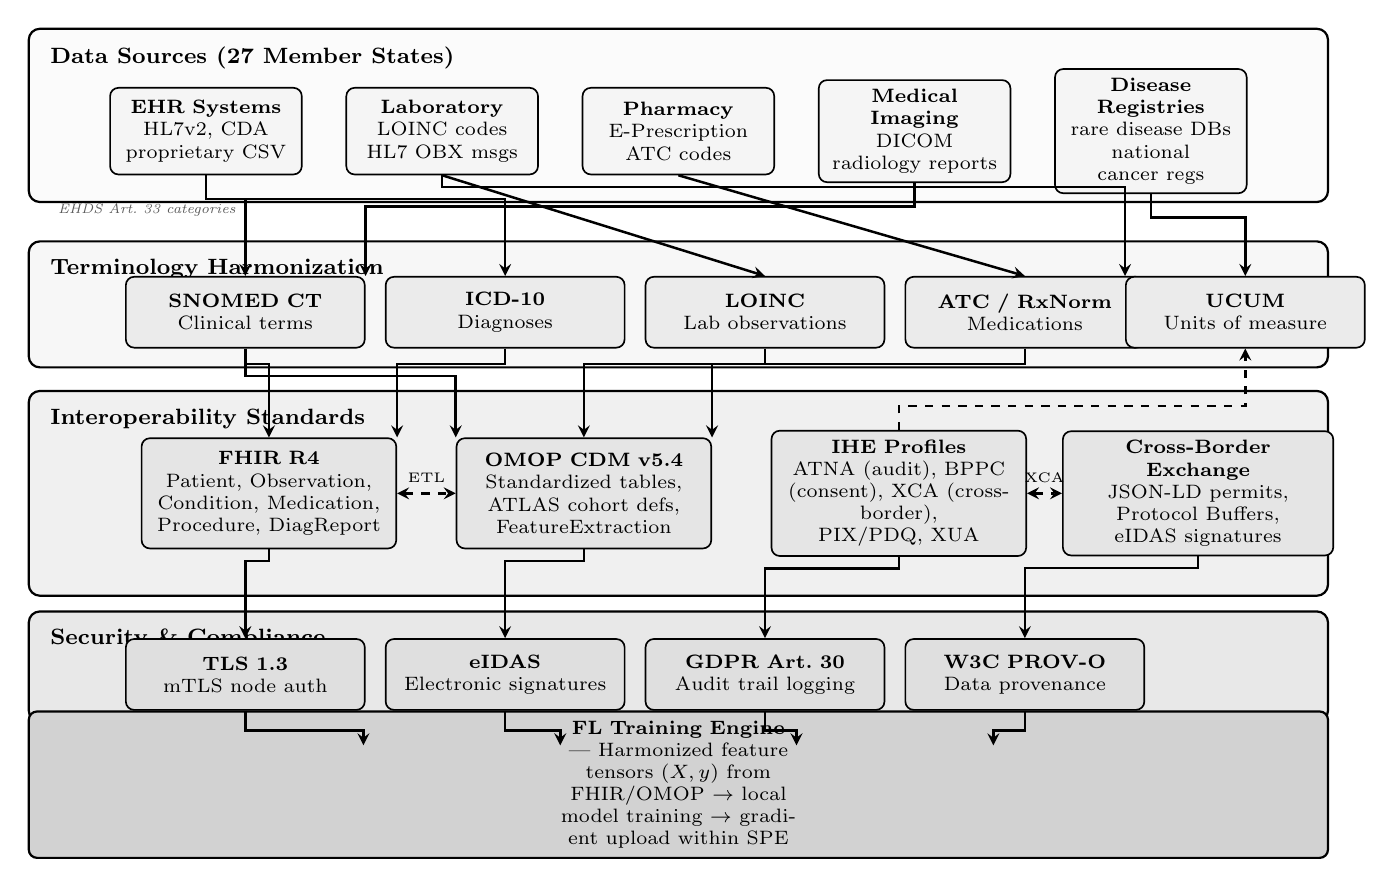
\begin{tikzpicture}[
    % Styles
    layer/.style={rectangle, rounded corners=4pt, draw=black, line width=0.8pt, minimum width=16.5cm},
    src/.style={rectangle, rounded corners=3pt, draw=black, line width=0.6pt, fill=gray!8, minimum height=1.1cm, text width=2.2cm, align=center, font=\scriptsize},
    std/.style={rectangle, rounded corners=3pt, draw=black, line width=0.6pt, fill=gray!20, minimum height=1.4cm, text width=3cm, align=center, font=\scriptsize},
    sec/.style={rectangle, rounded corners=3pt, draw=black, line width=0.6pt, fill=black!8, minimum height=0.9cm, text width=2.8cm, align=center, font=\scriptsize},
    flbox/.style={rectangle, rounded corners=3pt, draw=black, line width=0.8pt, fill=gray!30, minimum height=1.1cm, text width=3.2cm, align=center, font=\scriptsize},
    arrow/.style={->, >=stealth, line width=0.9pt},
    darrow/.style={->, >=stealth, line width=0.9pt, dashed},
    layerlabel/.style={font=\footnotesize\bfseries, anchor=north west},
]

% ===== LAYER A: DATA SOURCES =====
\node[layer, fill=gray!3, minimum height=2.2cm] (layerA) at (0, 7.2) {};
\node[layerlabel] at (-8.1, 8.2) {Data Sources (27 Member States)};

\node[src] (ehr) at (-6, 7.0) {\textbf{EHR Systems}\\HL7v2, CDA\\proprietary CSV};
\node[src] (lab) at (-3, 7.0) {\textbf{Laboratory}\\LOINC codes\\HL7 OBX msgs};
\node[src] (pharm) at (0, 7.0) {\textbf{Pharmacy}\\E-Prescription\\ATC codes};
\node[src] (img) at (3, 7.0) {\textbf{Medical Imaging}\\DICOM\\radiology reports};
\node[src] (reg) at (6, 7.0) {\textbf{Disease Registries}\\rare disease DBs\\national cancer regs};

% ===== LAYER B: TERMINOLOGY MAPPING =====
\node[layer, fill=gray!6, minimum height=1.6cm] (layerB) at (0, 4.8) {};
\node[layerlabel] at (-8.1, 5.5) {Terminology Harmonization};

\node[sec] (snomed) at (-5.5, 4.7) {\textbf{SNOMED CT}\\Clinical terms};
\node[sec] (icd10) at (-2.2, 4.7) {\textbf{ICD-10}\\Diagnoses};
\node[sec] (loinc) at (1.1, 4.7) {\textbf{LOINC}\\Lab observations};
\node[sec] (atc) at (4.4, 4.7) {\textbf{ATC / RxNorm}\\Medications};
\node[sec] (ucum) at (7.2, 4.7) {\textbf{UCUM}\\Units of measure};

% ===== LAYER C: INTEROPERABILITY STANDARDS =====
\node[layer, fill=gray!12, minimum height=2.6cm] (layerC) at (0, 2.4) {};
\node[layerlabel] at (-8.1, 3.6) {Interoperability Standards};

\node[std] (fhir) at (-5.2, 2.4) {\textbf{FHIR R4}\\Patient, Observation,\\Condition, Medication,\\Procedure, DiagReport};
\node[std] (omop) at (-1.2, 2.4) {\textbf{OMOP CDM v5.4}\\Standardized tables,\\ATLAS cohort defs,\\FeatureExtraction};
\node[std] (ihe) at (2.8, 2.4) {\textbf{IHE Profiles}\\ATNA (audit), BPPC\\(consent), XCA (cross-\\border), PIX/PDQ, XUA};
\node[std, text width=3.2cm] (xborder) at (6.6, 2.4) {\textbf{Cross-Border Exchange}\\JSON-LD permits,\\Protocol Buffers,\\eIDAS signatures};

% ===== LAYER D: SECURITY =====
\node[layer, fill=gray!18, minimum height=1.4cm] (layerD) at (0, 0.2) {};
\node[layerlabel] at (-8.1, 0.8) {Security \& Compliance};

\node[sec, fill=gray!25] (tls) at (-5.5, 0.1) {\textbf{TLS 1.3}\\mTLS node auth};
\node[sec, fill=gray!25] (eidas) at (-2.2, 0.1) {\textbf{eIDAS}\\Electronic signatures};
\node[sec, fill=gray!25] (gdpr) at (1.1, 0.1) {\textbf{GDPR Art.~30}\\Audit trail logging};
\node[sec, fill=gray!25] (prov) at (4.4, 0.1) {\textbf{W3C PROV-O}\\Data provenance};

% ===== FL ENGINE =====
\node[flbox, minimum width=16.5cm, minimum height=1cm, fill=gray!35] (fl) at (0, -1.3) {\textbf{FL Training Engine} --- Harmonized feature tensors $(X, y)$ from FHIR/OMOP $\to$ local model training $\to$ gradient upload within SPE};

% ===== ARROWS =====
% Sources to terminology
\draw[arrow] (ehr.south) -- ++(0,-0.3) -| (snomed.north);
\draw[arrow] (ehr.south) -- ++(0,-0.3) -| (icd10.north);
\draw[arrow] (lab.south) -- (loinc.north);
\draw[arrow] (pharm.south) -- (atc.north);
\draw[arrow] (img.south) -- ++(0,-0.3) -| (snomed.north east);
\draw[arrow] (reg.south) -- ++(0,-0.3) -| (ucum.north);
\draw[arrow] (lab.south) -- ++(0,-0.15) -| (ucum.north west);

% Terminology to standards
\draw[arrow] (snomed.south) -- ++(0,-0.2) -| (fhir.north);
\draw[arrow] (icd10.south) -- ++(0,-0.2) -| (fhir.north east);
\draw[arrow] (loinc.south) -- ++(0,-0.2) -| (omop.north);
\draw[arrow] (atc.south) -- ++(0,-0.2) -| (omop.north east);
\draw[arrow] (snomed.south) -- ++(0,-0.35) -| (omop.north west);
\draw[darrow] (ihe.north) -- ++(0, 0.3) -| (ucum.south);

% Standards to security
\draw[arrow] (fhir.south) -- ++(0,-0.15) -| (tls.north);
\draw[arrow] (omop.south) -- ++(0,-0.15) -| (eidas.north);
\draw[arrow] (ihe.south) -- ++(0,-0.15) -| (gdpr.north);
\draw[arrow] (xborder.south) -- ++(0,-0.15) -| (prov.north);

% Security to FL
\draw[arrow] (tls.south) -- ++(0, -0.25) -| (-4, -0.8);
\draw[arrow] (eidas.south) -- ++(0, -0.25) -| (-1.5, -0.8);
\draw[arrow] (gdpr.south) -- ++(0, -0.25) -| (1.5, -0.8);
\draw[arrow] (prov.south) -- ++(0, -0.25) -| (4, -0.8);

% Bidirectional between FHIR and OMOP
\draw[darrow, <->] (fhir.east) -- (omop.west) node[midway, above, font=\tiny] {ETL};

% Bidirectional between IHE and cross-border
\draw[darrow, <->] (ihe.east) -- (xborder.west) node[midway, above, font=\tiny] {XCA};

% EHDS Art 33 annotation
\node[font=\tiny\itshape, text=gray!70!black, anchor=west] at (-8, 6.0) {EHDS Art.~33 categories};

\end{tikzpicture}
\caption{EHDS interoperability architecture for FL-based secondary use. Data from heterogeneous sources across 27 Member States (top) flows through terminology harmonization (SNOMED CT, ICD-10, LOINC, ATC, UCUM), then through interoperability standards (FHIR R4 for structured data exchange, OMOP CDM for observational research, IHE profiles for cross-institutional workflows, cross-border exchange protocols with eIDAS signatures). A security and compliance layer enforces TLS~1.3 mutual authentication, eIDAS electronic signatures for permits, GDPR Article~30 audit logging, and W3C PROV-O data provenance before harmonized feature tensors reach the FL training engine. Bidirectional ETL between FHIR and OMOP enables institutions to use either standard based on their existing infrastructure.}
\label{fig:interop}
\end{figure*}

% ============================================================================
\section{Clinical Imaging: Extended Details}
\label{sec:imaging}
% ============================================================================

\subsection{Datasets}

Three clinical imaging datasets cover representative EHDS scenarios:
\begin{itemize}
    \item \textbf{Chest X-ray}~\cite{chestxray2018}: 5,860 pediatric radiographs (NORMAL/PNEUMONIA, 2.7:1 imbalance)
    \item \textbf{Brain Tumor MRI}: 3,064 T1-weighted CE MRI slices (3-class: glioma, meningioma, pituitary)
    \item \textbf{Skin Cancer}: 3,297 dermoscopy images (binary benign/malignant)
\end{itemize}

\subsection{Model Architectures}

\textbf{HealthcareResNet}: ResNet-18~\cite{he2016deep} pretrained on ImageNet, GroupNorm replacing BatchNorm for FL stability. FedBN~\cite{li2021fedbn} skips normalization during aggregation. Partial backbone freeze (level~1). $\sim$11.2M parameters.

\textbf{HealthcareCNN}: 5-block CNN with GroupNorm, progressive channels (32$\to$512), graduated Dropout (0.15$\to$0.3). Classifier: Flatten$\to$FC(512)$\to$FC(128)$\to$FC($K$). $\sim$12M parameters.

Data augmentation: random horizontal flip, rotation ($\pm$15\textdegree), brightness jitter ($\pm$10\%). ImageNet normalization.

\subsection{V2 Experimental Configuration}

\begin{itemize}
    \item 5 hospitals, 25 rounds, 3 local epochs, batch size 32
    \item Adam optimizer (lr=0.001), early stopping (patience=6)
    \item Non-IID via Dirichlet $\alpha{=}0.5$
    \item FedBN enabled, partial backbone freeze (level 1)
    \item 7 algorithms: FedAvg, FedProx, Ditto, FedLC, FedExP, FedLESAM, HPFL
    \item 3 seeds per configuration (42, 123, 456)
    \item Total: 7 $\times$ 5 datasets $\times$ 3 seeds = 105 experiments
\end{itemize}

\subsection{Reproducibility}

All experiments are fully reproducible:
\begin{verbatim}
cd fl-ehds-framework
# Full experiments (7 algo x 5 datasets x 3 seeds)
python -m benchmarks.run_full_experiments
# Quick validation (~1-2h)
python -m benchmarks.run_full_experiments --quick
# Resume after interruption
python -m benchmarks.run_full_experiments --resume
\end{verbatim}

Results, checkpoints, and logs are auto-saved to \texttt{benchmarks/paper\_results/}.

Repository: \url{https://github.com/FabioLiberti/FL-EHDS-FLICS2026}

% ============================================================================
\section{Detailed Architecture Description}
\label{sec:architecture_detail}
% ============================================================================

This section provides a comprehensive technical specification of the FL-EHDS three-layer architecture, detailing all modules, services, protocols, and standards implemented in the reference framework. Figure~\ref{fig:architecture} in the main paper provides the high-level view; Figure~\ref{fig:arch_detailed} presents the detailed component-level diagram; the description below enumerates every component with its specific technical parameters.

\begin{figure*}[t]
\centering
\includegraphics[width=\textwidth]{figures/fig_architecture_detailed.jpg}
\caption{FL-EHDS detailed architecture with component-level specifications. Layer~1 (Governance) includes four modules: HDAB Integration with OAuth2/mTLS authentication, Data Permit Manager (Article~53) with lifecycle management, Opt-Out Registry (Article~71) with LRU-cached filtering, and Cross-Border Coordinator (Articles~46, 50) with per-country privacy constraints. Layer~2 (FL Orchestration) operates within the Secure Processing Environment (SPE) with five modules: Aggregation Engine (17 FL algorithms), Privacy Protection (DP-SGD, Secure Aggregation, Byzantine Resilience), Compliance Module (GDPR audit logging), Communication Infrastructure (gRPC/WebSocket), and Monitoring \& Metrics. Layer~3 (Data Holders) implements a uniform stack per institution: Data Store, FHIR R4 Preprocessing, OMOP-CDM Harmonization, Local Training Engine, Gradient Processing, and Secure Communication. Inter-layer flows: Data Permit Authorization (OAuth2/mTLS, purpose-validated) downward from Layer~1; gradient upload (masked, encrypted, gRPC) upward and global model distribution (encrypted, TLS) downward between Layers~2--3.}
\label{fig:arch_detailed}
\end{figure*}

\subsection{Layer 1: Governance}

Four principal modules comprise the governance layer:

\textbf{1.1 HDAB Integration} (per Member State). Each Health Data Access Body instance implements: OAuth2/mTLS authentication with bearer token management (refresh tokens, scopes: \texttt{permits:read}, \texttt{permits:write}); a permit store with SQLite persistence backend; configurable HDAB strictness level (scale 1--5, where DE=5, ES=2); and national privacy constraints including per-jurisdiction differential privacy bounds ($\varepsilon_{\max}$: DE=1.0, FR=3.0, IT=5.0).

\textbf{1.2 Data Permit Manager} (Article~53). Manages the complete permit lifecycle: PENDING $\to$ APPROVED $\to$ ACTIVE $\to$ EXPIRED/REVOKED. Validates permitted purposes (scientific research, public health surveillance, AI system development, personalized medicine, official statistics) against authorized data categories (EHR, lab results, imaging, genomic, registry, ECG, pathology). Implements expiry verification and strict mode enforcement for continuous compliance.

\textbf{1.3 Opt-Out Registry} (Article~71). Supports three granularity levels: record-level, patient-level, and dataset-level opt-out. Registry lookups use LRU caching (max 100K records, TTL 10 min) with 300-second synchronization intervals to national registries. Configurable actions on opt-out match: exclude, anonymize, or error. Pre-training filtering ensures only opted-in data enters gradient computation.

\textbf{1.4 Cross-Border Coordinator} (Articles~46, 50). Implements multi-HDAB synchronization protocols across 10 pre-configured EU country profiles (DE, FR, IT, ES, NL, SE, PL, AT, BE, PT). Each profile specifies per-country constraints: $\varepsilon_{\max}$ for differential privacy, data retention periods (365--1,825 days), opt-out rates (3--12\%), and network latency characteristics (15--60ms based on geographic distance). The fee model (Article~42) implements cost-recovery calculation: base fee + per-record + per-round + per-MB charges.

\textbf{Inter-layer interface}: Data Permit Authorization (OAuth2/mTLS, purpose-validated, Articles~53+71) connects Layer~1 to Layer~2.

\subsection{Layer 2: FL Orchestration}

Five modules operate within the Secure Processing Environment (SPE), conforming to HealthData@EU infrastructure requirements:

\textbf{2.1 Aggregation Engine}. Implements 17 FL algorithms spanning six categories: \textit{Baseline} (FedAvg, FedProx with $\mu{=}0.01$, SCAFFOLD, FedNova, FedDyn); \textit{Adaptive} (FedAdam with server\_lr=0.1, FedYogi with $\beta_2{=}0.99$, FedAdagrad); \textit{Personalization} (Ditto with $\lambda{=}0.1$, Per-FedAvg via MAML, pFedMe, MOON); \textit{Non-IID} (FedLC for logit calibration, FedDecorr); \textit{SAM} (FedSAM, FedSpeed); \textit{Advanced} (FedExP ICLR'23, FedLESAM ICML'24, HPFL ICLR'25). Client selection strategies: random, performance-based, fairness-aware, latency-aware. Early stopping: patience=10, min\_delta=0.001. Model checkpointing with atomic saves.

\textbf{2.2 Privacy Protection Module}. Three sub-modules provide defense-in-depth:
\begin{itemize}
    \item \textit{DP-SGD}: Gaussian mechanism with R\'enyi DP (RDP) accounting. Configurable $\varepsilon$-budget (default 1.0), $\delta{=}10^{-5}$. Gradient clipping: max\_norm=1.0, type=L2/L$\infty$. RDP composition provides 5--6$\times$ tighter bounds than naive composition over 100+ rounds.
    \item \textit{Secure Aggregation}: Pairwise masking protocol with ECDH key exchange (SECP384R1 curve). Alternative protocols: Shamir secret sharing (threshold reconstruction), homomorphic encryption (CKKS scheme via TenSEAL). Dropout threshold: 50\%.
    \item \textit{Byzantine Resilience}: Six defense rules (Krum, Multi-Krum, Trimmed Mean, Coordinate-wise Median, Bulyan, FLTrust). Anomaly detection at 3$\sigma$ threshold. TEE integration for SGX/TrustZone hardware attestation.
\end{itemize}

\textbf{2.3 Compliance Module}. GDPR audit logging (Article~30) in JSON format with 7-year retention (2,555 days). Per-round purpose limitation check (Article~53). Opt-out enforcement: pre-training filtering combined with per-round verification. Anonymity assessment: $k$-anonymity, $l$-diversity checks. Automated EHDS compliance report with verification scoring.

\textbf{2.4 Communication Infrastructure}. gRPC bidirectional streaming for model updates (primary protocol). WebSocket for real-time monitoring and events. Compression: GZIP, LZ4, ZSTD, Snappy. Model chunking (ResNet-18: 44.7~MB/round $\to$ 8.9~MB with Top-$k$ 1\%). Security: TLS/mTLS with ECDHE key exchange. Retry: 3 attempts with 2$\times$ exponential backoff. Message types: MODEL\_UPDATE, GRADIENT\_UPDATE, HEARTBEAT, PERMIT\_VALIDATION, CONSENT\_CHECK, AUDIT\_LOG.

\textbf{2.5 Monitoring \& Metrics}. Tracks training convergence (accuracy, loss, F1, AUC per round), communication cost (MB/round), privacy budget consumption ($\varepsilon$ spent per round), participation statistics (samples, opt-outs), and resource utilization (CPU, memory, GPU). Structured logging via Structlog (JSON format) with Streamlit dashboard integration.

\textbf{Inter-module flows}: Privacy processing (DP-SGD, gradient clipping, secure masking) connects Aggregation $\to$ Privacy. Audit trail (GDPR Article~30, JSON logging, 7-year retention) connects Privacy $\to$ Compliance. Transport layer (gRPC streaming, TLS/mTLS, GZIP compression) connects Communication $\leftrightarrow$ all modules.

\subsection{Layer 3: Data Holders}

Each data holder institution (hospitals, disease registries, research centers across 27 Member States) implements a uniform component stack:

\textbf{3.1 Data Store}. Institutional health data in heterogeneous formats: EHR (FHIR R4), vitals (LOINC-coded), diagnoses (ICD-10 variants per country: ICD-10-GM for Germany, CIM-10 for France, ICD-9-CM legacy for Italy), ECG records (SCP-ECG standard EN~1064), and medical imaging (DICOM).

\textbf{3.2 FHIR R4 Preprocessing Engine}. Processes six FHIR resource types: Patient, Observation, Condition, MedicationRequest, Procedure, DiagnosticReport. Terminology mapping to international standards: SNOMED-CT (clinical concepts), LOINC (laboratory codes), ICD-10 (diagnoses), ATC (medications). Extracts 36 standardized features with normalization, encoding, and missing value imputation.

\textbf{3.3 OMOP-CDM Harmonizer}. Maps local vocabulary codes to standard OMOP Concept IDs. Populates OMOP tables: Person, ConditionOccurrence, Measurement, DrugExposure, ProcedureOccurrence, VisitOccurrence. Per-country vocabulary mapping ensures cross-border semantic compatibility.

\textbf{3.4 Local Training Engine}. Adaptive training with configurable parameters: optimizer (Adam, lr=0.001), batch size (32--256, dynamically adjusted), local epochs (3--5), dropout (0.3), L2 regularization. Device support: CUDA (GPU), MPS (Apple Silicon), CPU fallback for resource-constrained institutions.

\textbf{3.5 Gradient Processing}. Three-stage pipeline: (1)~gradient clipping (max\_norm=1.0, L2 norm); (2)~local DP noise addition (Gaussian, calibrated to $\varepsilon$); (3)~pairwise masking (ECDH shared keys with counterpart clients).

\textbf{3.6 Secure Communication}. AES-256-GCM symmetric encryption for gradient payloads. ECDHE key exchange (SECP384R1 curve). mTLS mutual authentication with certificate-based identity. Nonce generation for replay attack prevention.

\textbf{Inter-layer data flow}: Gradient upload ($\nabla$ masked, encrypted, gRPC) flows upward from Layer~3 to Layer~2. Global model distribution ($\theta$ encrypted, TLS) flows downward from Layer~2 to Layer~3.

\textbf{Architectural invariant}: Raw health data never leaves institutional boundaries---only encrypted model gradients are exchanged within the Secure Processing Environment.

% ============================================================================
\section{Extended Tabular Experiment Results}
\label{sec:extended_tabular}
% ============================================================================

This section presents comprehensive experimental results from 731 federated learning experiments across three tabular healthcare datasets: PTB-XL ECG (21,799 records, 52 European recording sites, 5-class cardiac diagnosis), Cardiovascular Disease (70,000 patients, binary classification), and Breast Cancer Wisconsin (569 samples, binary classification). The evaluation comprises a baseline comparison (63 experiments, 7 algorithms $\times$ 3 datasets $\times$ 3 seeds) and three sweep phases: heterogeneity ($\alpha$ variation, 252 experiments), client scaling (189 experiments), and learning rate sensitivity (108 experiments). All results are reproducible via the benchmark suite.

\subsection{Heterogeneity Impact}

Table~\ref{tab:heterogeneity} shows accuracy as a function of Dirichlet $\alpha$ (lower $\alpha$ = more non-IID). The ``Site'' column reports natural site-based partitioning for PTB-XL.

\begin{table*}[t]
\centering
\caption{Impact of data heterogeneity ($\alpha$) on FL accuracy (\%). Lower $\alpha$ = more non-IID. Mean over 3 seeds. PX = PTB-XL, CV = Cardiovascular, BC = Breast Cancer.}
\label{tab:heterogeneity}
\small
\begin{tabular}{llcccccc}
\toprule
\textbf{DS} & \textbf{Algorithm} & \textbf{IID} & \textbf{$\alpha$=0.1} & \textbf{$\alpha$=0.3} & \textbf{$\alpha$=0.5} & \textbf{$\alpha$=1.0} & \textbf{Site} \\
\midrule
PX & FedAvg & 90.8 & 88.9 & 91.3 & 91.1 & 91.9 & 92.0 \\
 & FedProx & 91.1 & 88.8 & 91.3 & 91.1 & 91.9 & 91.6 \\
 & Ditto & 91.9 & \textbf{96.4} & \textbf{96.6} & \textbf{95.4} & 93.3 & 91.8 \\
 & FedLC & 90.8 & 88.9 & 91.3 & 90.6 & 91.4 & 92.0 \\
 & FedExP & 90.8 & 88.9 & 91.3 & 91.1 & 91.9 & 92.0 \\
 & FedLESAM & 90.8 & 88.9 & 91.3 & 91.1 & 91.9 & 92.0 \\
 & HPFL & 91.8 & 96.3 & 96.0 & 94.9 & \textbf{93.8} & \textbf{92.6} \\
\midrule
CV & FedAvg & 72.6 & 60.7 & 63.3 & 71.0 & 72.6 & -- \\
 & FedProx & 72.6 & 60.9 & 63.2 & 71.4 & 72.6 & -- \\
 & Ditto & 72.7 & \textbf{89.3} & \textbf{91.5} & 81.7 & 81.4 & -- \\
 & FedLC & 72.6 & 60.9 & 63.5 & 70.8 & 72.6 & -- \\
 & FedExP & 72.6 & 60.7 & 63.4 & 71.0 & 72.6 & -- \\
 & FedLESAM & 72.6 & 60.7 & 63.4 & 71.0 & 72.6 & -- \\
 & HPFL & \textbf{72.6} & 89.2 & 91.5 & \textbf{81.7} & \textbf{81.2} & -- \\
\midrule
BC & FedAvg & 58.7 & 72.6 & 59.6 & 61.1 & 60.4 & -- \\
 & FedProx & 58.7 & 72.6 & 59.6 & 61.1 & 60.4 & -- \\
 & Ditto & 59.6 & 80.5 & 81.4 & 79.9 & 71.9 & -- \\
 & FedLC & 59.0 & 72.6 & 59.3 & 61.1 & 60.4 & -- \\
 & FedExP & 58.7 & 72.6 & 59.6 & 61.1 & 60.4 & -- \\
 & FedLESAM & 58.7 & 72.6 & 59.6 & 61.1 & 60.4 & -- \\
 & HPFL & 59.9 & \textbf{80.5} & \textbf{81.4} & \textbf{80.5} & \textbf{71.9} & -- \\
\bottomrule
\end{tabular}
\end{table*}

\textbf{Key finding}: Personalized algorithms (Ditto, HPFL) exhibit a counter-intuitive pattern: accuracy \textit{increases} under extreme non-IID ($\alpha{=}0.1$) on Cardiovascular (89.3\% vs.\ 81.7\% at $\alpha{=}0.5$) and Breast Cancer (80.5\% vs.\ 79.9\%). This occurs because personalized methods maintain local decision boundaries that become more specialized---and therefore more accurate---when client distributions are highly distinct. In contrast, baseline algorithms (FedAvg, FedExP, FedLESAM) degrade monotonically as $\alpha$ decreases, consistent with theoretical predictions. For PTB-XL, natural site-based partitioning produces the most realistic non-IID conditions and yields strong performance across all algorithms (88.9--96.6\%).

\subsection{Client Scaling}

Table~\ref{tab:client_scaling} reports accuracy as a function of client count $K$.

\begin{table*}[t]
\centering
\caption{Impact of client count on FL accuracy (\%). Mean over 3 seeds. PX = PTB-XL, CV = Cardiovascular, BC = Breast Cancer.}
\label{tab:client_scaling}
\small
\begin{tabular}{lcccc}
\toprule
\multicolumn{5}{c}{\textbf{PTB-XL ECG (5-class)}} \\
\textbf{Algorithm} & \textbf{K=3} & \textbf{K=5} & \textbf{K=10} & \textbf{K=20} \\
\midrule
FedAvg & 91.5 & 92.0 & 91.5 & 91.5 \\
FedProx & 91.5 & 91.6 & 91.5 & 91.5 \\
Ditto & \textbf{92.5} & 91.8 & 91.4 & 91.4 \\
FedLC & 92.1 & 92.0 & 92.0 & 92.0 \\
FedExP & 91.5 & 92.0 & 92.2 & \textbf{92.2} \\
FedLESAM & 91.5 & 92.0 & 91.5 & 91.5 \\
HPFL & \textbf{92.6} & \textbf{92.6} & \textbf{92.4} & \textbf{92.4} \\
\bottomrule
\end{tabular}
\hspace{3mm}
\begin{tabular}{lcccc}
\toprule
\multicolumn{5}{c}{\textbf{Cardiovascular (binary)}} \\
\textbf{Algorithm} & \textbf{K=3} & \textbf{K=5} & \textbf{K=8} & \textbf{K=10} \\
\midrule
FedAvg & 71.9 & 71.0 & 69.2 & 67.3 \\
FedProx & 72.0 & 71.4 & 69.6 & 67.7 \\
Ditto & 78.5 & 81.7 & 84.2 & \textbf{87.3} \\
FedLC & 71.9 & 70.8 & 69.5 & 66.4 \\
FedExP & 71.9 & 71.0 & 69.2 & 67.3 \\
FedLESAM & 71.9 & 71.0 & 69.2 & 67.3 \\
HPFL & \textbf{78.6} & \textbf{81.7} & \textbf{84.1} & 86.7 \\
\bottomrule
\end{tabular}
\hspace{3mm}
\begin{tabular}{lccc}
\toprule
\multicolumn{4}{c}{\textbf{Breast Cancer (binary)}} \\
\textbf{Algorithm} & \textbf{K=2} & \textbf{K=3} & \textbf{K=5} \\
\midrule
FedAvg & 68.1 & 61.1 & 58.3 \\
FedProx & 68.1 & 61.1 & 58.3 \\
Ditto & \textbf{82.9} & 79.9 & 76.2 \\
FedLC & 59.9 & 61.1 & 58.6 \\
FedExP & 68.1 & 61.1 & 58.3 \\
FedLESAM & 68.1 & 61.1 & 58.3 \\
HPFL & \textbf{82.9} & \textbf{80.5} & \textbf{76.2} \\
\bottomrule
\end{tabular}
\end{table*}

\textbf{Key finding}: Baseline algorithms (FedAvg, FedExP, FedLESAM) degrade as client count increases on Cardiovascular (71.9\% at K=3 $\to$ 67.3\% at K=10), because more clients means less data per client and higher aggregation noise. Personalized methods show the opposite trend: Ditto \textit{improves} from 78.5\% (K=3) to 87.3\% (K=10), demonstrating that personalization enables each client to exploit its local specialization even with smaller data partitions. This has direct EHDS implications: as more Member States join a federation, personalized algorithms become increasingly advantageous.

\subsection{Learning Rate Sensitivity}

Table~\ref{tab:lr_sensitivity} evaluates robustness to learning rate selection for the top-3 algorithms.

\begin{table}[t]
\centering
\caption{Learning rate sensitivity analysis. Accuracy (\%) mean over 3 seeds. Top-3 algorithms: HPFL, Ditto, FedAvg.}
\label{tab:lr_sensitivity}
\small
\begin{tabular}{llcccc}
\toprule
\textbf{DS} & \textbf{Algo} & \textbf{0.0005} & \textbf{0.001} & \textbf{0.005} & \textbf{0.01} \\
\midrule
PX & Ditto & 56.5 & 83.4 & 91.8 & 92.6 \\
 & FedAvg & 78.9 & 89.9 & 92.0 & 92.2 \\
 & HPFL & 61.2 & 86.8 & 92.6 & \textbf{92.7} \\
\midrule
CV & Ditto & 74.3 & 75.4 & 81.6 & \textbf{81.7} \\
 & FedAvg & 50.2 & 55.4 & 71.2 & 71.0 \\
 & HPFL & 74.3 & 75.1 & \textbf{81.7} & \textbf{81.7} \\
\midrule
BC & Ditto & 80.8 & 79.9 & \textbf{95.9} & \textbf{95.9} \\
 & FedAvg & 61.1 & 61.1 & 66.1 & 64.9 \\
 & HPFL & 80.5 & 80.5 & \textbf{96.2} & 95.9 \\
\bottomrule
\end{tabular}
\end{table}

\textbf{Key finding}: All algorithms are sensitive to learning rate at the low end (lr=0.0005), where convergence is incomplete within the configured round budget. HPFL and Ditto achieve near-optimal performance across a wider range (0.005--0.01), while FedAvg requires careful tuning. On Breast Cancer, HPFL reaches 96.2\% accuracy at lr=0.005---substantially higher than the baseline configuration (80.5\% at lr=0.001)---suggesting that per-dataset hyperparameter optimization is critical for small datasets.

\subsection{Fairness Analysis}

Table~\ref{tab:fairness_detail} provides per-client fairness metrics across all datasets.

\begin{table}[t]
\centering
\caption{Per-client fairness analysis. Gap = max--min client accuracy. Lower Gap and Gini indicate fairer distribution.}
\label{tab:fairness_detail}
\footnotesize
\begin{tabular}{ll cccc}
\toprule
\textbf{DS} & \textbf{Algo} & \textbf{Jain} & \textbf{Gini} & \textbf{Gap (\%)} & \textbf{Std (\%)} \\
\midrule
PX & FedAvg & 0.999 & 0.012 & 6.7 & 2.3 \\
 & FedProx & 0.999 & 0.010 & 5.2 & 1.8 \\
 & Ditto & 0.999 & 0.013 & 6.2 & 2.2 \\
 & HPFL & 0.999 & 0.019 & 9.7 & 3.4 \\
\midrule
CV & FedAvg & 0.982 & 0.063 & 22.6 & 8.6 \\
 & FedProx & 0.985 & 0.058 & 21.0 & 7.9 \\
 & Ditto & 0.984 & 0.062 & 22.7 & 8.6 \\
 & HPFL & 0.984 & 0.069 & 26.1 & 11.2 \\
\midrule
BC & FedAvg & 0.536 & 0.473 & 87.6 & 40.0 \\
 & Ditto & 0.536 & 0.473 & 87.6 & 40.0 \\
 & HPFL & \textbf{0.785} & \textbf{0.230} & \textbf{70.5} & \textbf{33.1} \\
\bottomrule
\end{tabular}
\end{table}

\textbf{Key finding}: HPFL uniquely improves fairness on Breast Cancer (Jain 0.785 vs.\ 0.536 for all other algorithms, Gini reduction from 0.473 to 0.230). This occurs because HPFL's personalized classifier heads enable each client to specialize, reducing the performance gap between clients with different class distributions. On PTB-XL, all algorithms achieve near-perfect fairness (Jain $\geq$ 0.999) due to the large dataset size providing sufficient per-client samples.

\subsection{Statistical Significance}

Table~\ref{tab:significance} reports Wilcoxon signed-rank test $p$-values comparing each algorithm against FedAvg.

\begin{table}[t]
\centering
\caption{Wilcoxon signed-rank $p$-values vs FedAvg baseline. $\dagger$: $p < 0.05$.}
\label{tab:significance}
\small
\begin{tabular}{lccc}
\toprule
\textbf{vs FedAvg} & \textbf{PX} & \textbf{CV} & \textbf{BC} \\
\midrule
FedProx & 0.250 & 1.000 & 1.000 \\
Ditto & 0.250 & 0.250 & 0.250 \\
FedLC & 1.000 & 0.750 & 1.000 \\
FedExP & 0.750 & 1.000 & 1.000 \\
FedLESAM & 1.000 & 1.000 & 1.000 \\
HPFL & 0.250 & 0.250 & 0.250 \\
\bottomrule
\end{tabular}
\end{table}

\textbf{Note}: With only 3 seeds, the minimum achievable $p$-value for Wilcoxon is 0.250, insufficient for conventional significance thresholds. The consistent directional advantage of HPFL and Ditto across all datasets (effect sizes of 10--19pp on Cardiovascular and Breast Cancer) provides practical significance despite the limited seed count. Extended evaluation with additional seeds is planned as future work.

\subsection{Experimental Configuration Summary}

\begin{table}[t]
\centering
\caption{Per-dataset optimal configuration.}
\label{tab:dataset_config}
\small
\begin{tabular}{lcccccc}
\toprule
\textbf{Dataset} & \textbf{lr} & \textbf{bs} & \textbf{rounds} & \textbf{K} & \textbf{$\alpha$} & \textbf{Partition} \\
\midrule
PTB-XL & 0.005 & 64 & 30 & 5 & -- & Site-based \\
Cardiovascular & 0.01 & 64 & 25 & 5 & 0.5 & Dirichlet \\
Breast Cancer & 0.001 & 16 & 40 & 3 & 0.5 & Dirichlet \\
\bottomrule
\end{tabular}
\end{table}

\textbf{Reproducibility}: All experiments are fully reproducible via:
\begin{verbatim}
cd fl-ehds-framework
# Baseline (63 experiments, ~27 min)
python -m benchmarks.run_tabular_optimized
# Multi-phase sweep (668 experiments, ~3.2h)
python -m benchmarks.run_tabular_sweep --phase all
# Extended analysis (tables + plots)
python -m benchmarks.analyze_tabular_extended
\end{verbatim}

Results, checkpoints, and analysis outputs are auto-saved to \texttt{benchmarks/paper\_results\_tabular/}.

\subsection{Extended Tabular Experiment Figures}

Figures~\ref{fig:tab_convergence}--\ref{fig:tab_best_config} present visual analysis of the 731 tabular experiments. All plots are auto-generated by the benchmark analysis suite.

\begin{figure}[htbp]
\centering
\includegraphics[width=0.95\columnwidth]{figures/00_convergence_accuracy.pdf}
\caption{Training convergence curves (accuracy vs.\ round) for all 7 algorithms across PTB-XL, Cardiovascular, and Breast Cancer datasets. HPFL and Ditto converge faster and to higher accuracy on all datasets.}
\label{fig:tab_convergence}
\end{figure}

\begin{figure}[htbp]
\centering
\includegraphics[width=0.95\columnwidth]{figures/01_accuracy_bars.pdf}
\caption{Final accuracy comparison across algorithms and datasets. Error bars show standard deviation over 3 seeds. HPFL achieves the best accuracy on all three datasets.}
\label{fig:tab_accuracy_bars}
\end{figure}

\begin{figure}[htbp]
\centering
\includegraphics[width=0.95\columnwidth]{figures/02_fairness_bars.pdf}
\caption{Jain fairness index per algorithm and dataset. PTB-XL achieves near-perfect fairness (0.999) across all algorithms. HPFL uniquely improves fairness on Breast Cancer (0.785 vs.\ 0.536).}
\label{fig:tab_fairness_bars}
\end{figure}

\begin{figure}[htbp]
\centering
\includegraphics[width=0.95\columnwidth]{figures/03_accuracy_boxplots.pdf}
\caption{Accuracy distribution across seeds and datasets. Box plots show median, quartiles, and outliers. Ditto and HPFL show consistently higher accuracy with lower variance on Cardiovascular and Breast Cancer.}
\label{fig:tab_boxplots}
\end{figure}

\begin{figure}[htbp]
\centering
\includegraphics[width=0.95\columnwidth]{figures/04_client_heatmaps.pdf}
\caption{Per-client accuracy heatmaps. Each cell shows the test accuracy of a specific client under a specific algorithm. Reveals client-level heterogeneity patterns across datasets.}
\label{fig:tab_client_heatmaps}
\end{figure}

\begin{figure}[htbp]
\centering
\includegraphics[width=0.95\columnwidth]{figures/05_loss_convergence.pdf}
\caption{Training loss convergence curves. Lower is better. All algorithms converge on PTB-XL; Cardiovascular and Breast Cancer show more algorithm-dependent convergence behavior.}
\label{fig:tab_loss_convergence}
\end{figure}

\begin{figure}[htbp]
\centering
\includegraphics[width=0.95\columnwidth]{figures/06_f1_convergence.pdf}
\caption{F1-score convergence over training rounds. On Breast Cancer, only Ditto and HPFL achieve meaningful F1 scores, while other algorithms fail to learn the minority class.}
\label{fig:tab_f1_convergence}
\end{figure}

\begin{figure}[htbp]
\centering
\includegraphics[width=0.95\columnwidth]{figures/07_rounds_to_converge.pdf}
\caption{Rounds to convergence (defined as 95\% of final accuracy). Earlier convergence reduces communication cost. HPFL and Ditto converge in fewer rounds on Cardiovascular.}
\label{fig:tab_rounds_converge}
\end{figure}

\begin{figure}[htbp]
\centering
\includegraphics[width=0.95\columnwidth]{figures/08_accuracy_vs_fairness.pdf}
\caption{Accuracy vs.\ fairness (Jain index) scatter plot. The ideal position is the top-right corner (high accuracy, high fairness). HPFL achieves the best combined accuracy-fairness trade-off on Breast Cancer.}
\label{fig:tab_acc_fairness}
\end{figure}

\begin{figure}[htbp]
\centering
\includegraphics[width=0.95\columnwidth]{figures/09_radar_charts.pdf}
\caption{Multi-metric radar charts per algorithm (accuracy, F1, Jain, convergence speed, communication efficiency). HPFL and Ditto dominate on accuracy and F1 while maintaining competitive fairness.}
\label{fig:tab_radar}
\end{figure}

\begin{figure}[htbp]
\centering
\includegraphics[width=0.95\columnwidth]{figures/10_data_distribution.pdf}
\caption{Data distribution across clients after Dirichlet partitioning. Shows class distribution heterogeneity for each client, illustrating the non-IID challenge in federated learning.}
\label{fig:tab_data_dist}
\end{figure}

\begin{figure}[htbp]
\centering
\includegraphics[width=0.95\columnwidth]{figures/11_ranking_heatmap.pdf}
\caption{Algorithm ranking heatmap across datasets and metrics. Each cell shows the rank (1=best, 7=worst) of each algorithm. HPFL ranks first on all datasets; Ditto consistently ranks second.}
\label{fig:tab_ranking}
\end{figure}

\begin{figure}[htbp]
\centering
\includegraphics[width=0.95\columnwidth]{figures/12_early_stopping.pdf}
\caption{Early stopping analysis: actual rounds used vs.\ configured maximum. Most algorithms converge before the maximum round budget, demonstrating the effectiveness of patience-based early stopping.}
\label{fig:tab_early_stopping}
\end{figure}

\begin{figure}[htbp]
\centering
\includegraphics[width=0.95\columnwidth]{figures/13_runtime.pdf}
\caption{Wall-clock training time per algorithm and dataset. PTB-XL requires 12--40s depending on algorithm. Cardiovascular (70K samples) requires 38--100s. Breast Cancer is near-instantaneous ($<$1s).}
\label{fig:tab_runtime}
\end{figure}

\begin{figure}[htbp]
\centering
\includegraphics[width=0.95\columnwidth]{figures/14_heterogeneity_impact.pdf}
\caption{Impact of data heterogeneity ($\alpha$) on accuracy. Line plot showing accuracy vs.\ Dirichlet $\alpha$ for each algorithm. Personalized methods (Ditto, HPFL) improve under extreme non-IID ($\alpha{=}0.1$).}
\label{fig:tab_hetero_impact}
\end{figure}

\begin{figure}[htbp]
\centering
\includegraphics[width=0.95\columnwidth]{figures/15_heterogeneity_heatmap.pdf}
\caption{Heterogeneity sweep heatmap: algorithm $\times$ $\alpha$ per dataset. Color intensity represents accuracy. Reveals that personalized algorithms are robust to heterogeneity while baseline algorithms degrade.}
\label{fig:tab_hetero_heatmap}
\end{figure}

\begin{figure}[htbp]
\centering
\includegraphics[width=0.95\columnwidth]{figures/16_client_scaling.pdf}
\caption{Client scaling analysis: accuracy vs.\ number of clients $K$. Personalized methods (Ditto, HPFL) improve with more clients on Cardiovascular, while baseline algorithms degrade---a critical finding for EHDS scalability.}
\label{fig:tab_client_scaling}
\end{figure}

\begin{figure}[htbp]
\centering
\includegraphics[width=0.95\columnwidth]{figures/17_client_scaling_fairness.pdf}
\caption{Fairness (Jain index) vs.\ client count. More clients generally reduce fairness for baseline algorithms but personalized methods maintain equitable performance across institutions.}
\label{fig:tab_scaling_fairness}
\end{figure}

\begin{figure}[htbp]
\centering
\includegraphics[width=0.95\columnwidth]{figures/18_lr_sensitivity.pdf}
\caption{Learning rate sensitivity for top-3 algorithms (HPFL, Ditto, FedAvg). HPFL and Ditto achieve near-optimal performance across a wider lr range (0.005--0.01) compared to FedAvg.}
\label{fig:tab_lr_sensitivity}
\end{figure}

\begin{figure}[htbp]
\centering
\includegraphics[width=0.95\columnwidth]{figures/19_ptbxl_site_vs_dirichlet.pdf}
\caption{PTB-XL: natural site-based vs.\ synthetic Dirichlet partitioning comparison. Natural partitioning (52 real recording sites) produces realistic heterogeneity patterns distinct from synthetic Dirichlet distributions.}
\label{fig:tab_ptbxl_partition}
\end{figure}

\begin{figure}[htbp]
\centering
\includegraphics[width=0.95\columnwidth]{figures/20_algorithm_grid.pdf}
\caption{Algorithm comparison grid: 3 metrics (accuracy, F1, Jain) $\times$ 3 datasets. Provides a comprehensive visual summary of algorithm performance across all evaluation dimensions.}
\label{fig:tab_algo_grid}
\end{figure}

\begin{figure}[htbp]
\centering
\includegraphics[width=0.95\columnwidth]{figures/21_best_config_summary.pdf}
\caption{Best configuration summary per dataset. Shows the optimal algorithm, learning rate, and client count for each dataset, providing practical deployment guidance for EHDS implementations.}
\label{fig:tab_best_config}
\end{figure}

% ============================================================================
\bibliographystyle{IEEEtran}
% Bibliography synchronized with main paper (48 entries)
\begin{thebibliography}{48}

% === EHDS Regulation and Policy ===
\bibitem{eu2025ehds}
European Commission, ``Regulation (EU) 2025/327 on the European Health Data Space,'' \textit{Official Journal of the EU}, L 2025/327, Mar. 2025.

\bibitem{staunton2024ethical}
C. Staunton \textit{et al.}, ``Ethical and social reflections on the proposed European Health Data Space,'' \textit{Eur.~J.~Human Genetics}, vol.~32, no.~5, pp.~498--505, 2024.

\bibitem{quinn2024gdpr}
P. Quinn, E. Ellyne, and C. Yao, ``Will the GDPR restrain health data access bodies under the EHDS?'' \textit{Computer Law \& Security Review}, vol.~54, art.~105993, 2024.

\bibitem{tehdas2024ready}
TEHDAS Joint Action, ``Are EU member states ready for the European Health Data Space?'' \textit{Eur.~J.~Public Health}, vol.~34, no.~6, pp.~1102--1108, 2024.

\bibitem{frohlich2025reality}
H. Fr\"ohlich \textit{et al.}, ``Reality check: The aspirations of the EHDS amidst challenges in decentralized data analysis,'' \textit{J.~Med.~Internet Res.}, vol.~27, art.~e76491, 2025.

\bibitem{vandrumpt2025pets}
S. van Drumpt \textit{et al.}, ``Secondary use under the European Health Data Space,'' \textit{Frontiers in Digital Health}, vol.~7, art.~1602101, 2025.

\bibitem{hussein2025interop}
R. Hussein \textit{et al.}, ``Interoperability framework of the EHDS for secondary use,'' \textit{J.~Med.~Internet Res.}, vol.~27, art.~e69813, 2025.

\bibitem{forster2025journeys}
R. Forster \textit{et al.}, ``User journeys in cross-European secondary use of health data,'' \textit{Eur.~J.~Public Health}, vol.~35, Suppl.~3, pp.~iii18--iii24, 2025.

\bibitem{svingel2025hdab}
L. Svingel \textit{et al.}, ``Shaping the future EHDS: Recommendations for HDABs,'' \textit{Eur.~J.~Public Health}, vol.~35, Suppl.~3, pp.~iii32--iii38, 2025.

\bibitem{christiansen2025pilot}
C. Christiansen \textit{et al.}, ``Piloting an infrastructure for secondary use of health data,'' \textit{Eur.~J.~Public Health}, vol.~35, Suppl.~3, pp.~iii3--iii4, 2025.

\bibitem{shabani2024ehds}
M. Shabani and P. Borry, ``The European Health Data Space: Challenges and opportunities,'' \textit{Eur.~J.~Human Genetics}, vol.~32, no.~8, pp.~891--897, 2024.

\bibitem{ganna2024boost}
A. Ganna, E. Ingelsson, and D. Posthuma, ``The EHDS can be a boost for research beyond borders,'' \textit{Nature Medicine}, vol.~30, pp.~3053--3056, 2024.

% === FL Foundations ===
\bibitem{mcmahan2017communication}
B. McMahan \textit{et al.}, ``Communication-efficient learning of deep networks from decentralized data,'' in \textit{Proc. AISTATS}, pp.~1273--1282, 2017.

\bibitem{li2020federated}
T. Li \textit{et al.}, ``Federated optimization in heterogeneous networks,'' in \textit{Proc. MLSys}, vol.~2, pp.~429--450, 2020.

\bibitem{kairouz2021advances}
P. Kairouz \textit{et al.}, ``Advances and open problems in federated learning,'' \textit{Found.~Trends Mach.~Learn.}, vol.~14, no.~1--2, pp.~1--210, 2021.

\bibitem{rieke2020future}
N. Rieke \textit{et al.}, ``The future of digital health with federated learning,'' \textit{npj Digital Medicine}, vol.~3, art.~119, 2020.

\bibitem{bonawitz2019scale}
K. Bonawitz \textit{et al.}, ``Towards federated learning at scale,'' in \textit{Proc. MLSys}, pp.~374--388, 2019.

\bibitem{chaverodiez2026fair}
M. Chavero-Diez \textit{et al.}, ``Federated learning frameworks: Quality and interoperability for biomedical research,'' \textit{NAR Genomics Bioinformatics}, vol.~8, no.~1, art.~lqag010, 2026.

% === FL Reviews ===
\bibitem{teo2024systematic}
Z. L. Teo \textit{et al.}, ``Federated machine learning in healthcare: A systematic review,'' \textit{Cell Reports Medicine}, vol.~5, no.~2, art.~101419, 2024.

\bibitem{peng2024systematic}
L. Peng \textit{et al.}, ``Federated machine learning in healthcare: A systematic review,'' \textit{Comput.~Methods Programs Biomed.}, vol.~247, art.~108066, 2024.

% === Privacy and Security ===
\bibitem{zhu2019deep}
L. Zhu, Z. Liu, and S. Han, ``Deep leakage from gradients,'' in \textit{Proc. NeurIPS}, vol.~32, pp.~14774--14784, 2019.

\bibitem{shokri2017membership}
R. Shokri \textit{et al.}, ``Membership inference attacks against machine learning models,'' in \textit{Proc. IEEE S\&P}, pp.~3--18, 2017.

\bibitem{carlini2022privacy}
N. Carlini \textit{et al.}, ``Membership inference attacks from first principles,'' in \textit{Proc. IEEE S\&P}, pp.~1897--1914, 2022.

\bibitem{dwork2014dp}
C. Dwork and A. Roth, ``The algorithmic foundations of differential privacy,'' \textit{Found.~Trends Theor.~Comput.~Sci.}, vol.~9, no.~3--4, pp.~211--407, 2014.

\bibitem{abadi2016deep}
M. Abadi \textit{et al.}, ``Deep learning with differential privacy,'' in \textit{Proc. ACM CCS}, pp.~308--318, 2016.

\bibitem{mironov2017renyi}
I. Mironov, ``R\'enyi differential privacy,'' in \textit{Proc. IEEE CSF}, pp.~263--275, 2017.

\bibitem{wei2020federated}
K. Wei \textit{et al.}, ``Federated learning with differential privacy,'' \textit{IEEE Trans.~Inf.~Forensics Secur.}, vol.~15, pp.~3454--3469, 2020.

\bibitem{jordon2022synthetic}
J. Jordon \textit{et al.}, ``Synthetic data---A privacy mirage?'' \textit{J.~Mach.~Learn.~Res.}, vol.~23, no.~1, art.~298, 2022.

% === FL Healthcare ===
\bibitem{dayan2021federated}
I. Dayan \textit{et al.}, ``Federated learning for predicting clinical outcomes in patients with COVID-19,'' \textit{Nature Medicine}, vol.~27, no.~10, pp.~1735--1743, 2021.

\bibitem{sheller2020federated}
M. J. Sheller \textit{et al.}, ``Federated learning in medicine,'' \textit{Scientific Reports}, vol.~10, art.~12598, 2020.

% === FL Algorithms ===
\bibitem{karimireddy2020scaffold}
S. P. Karimireddy \textit{et al.}, ``SCAFFOLD: Stochastic controlled averaging for federated learning,'' in \textit{Proc. ICML}, pp.~5132--5143, 2020.

\bibitem{wang2020tackling}
J. Wang \textit{et al.}, ``Tackling the objective inconsistency problem in heterogeneous federated optimization,'' in \textit{Proc. NeurIPS}, vol.~33, pp.~7611--7623, 2020.

\bibitem{reddi2021adaptive}
S. Reddi \textit{et al.}, ``Adaptive federated optimization,'' in \textit{Proc. ICLR}, 2021.

\bibitem{li2021ditto}
T. Li \textit{et al.}, ``Ditto: Fair and robust federated learning through personalization,'' in \textit{Proc. ICML}, PMLR 139, pp.~6357--6368, 2021.

\bibitem{fallah2020personalized}
A. Fallah, A. Mokhtari, and A. Ozdaglar, ``Personalized federated learning with Moreau envelopes,'' in \textit{Proc. NeurIPS}, vol.~33, pp.~21394--21405, 2020.

\bibitem{qu2022fedsam}
Z. Qu \textit{et al.}, ``Generalized federated learning via sharpness aware minimization,'' in \textit{Proc. ICML}, PMLR 162, pp.~18250--18280, 2022.

\bibitem{zhang2022fedlc}
J. Zhang \textit{et al.}, ``Federated learning with label distribution skew via logits calibration,'' in \textit{Proc. ICML}, PMLR 162, pp.~26311--26329, 2022.

\bibitem{shi2023feddecorr}
Y. Shi \textit{et al.}, ``Towards understanding and mitigating dimensional collapse in heterogeneous federated learning,'' in \textit{Proc. ICLR}, 2023.

\bibitem{sun2023fedspeed}
Y. Sun \textit{et al.}, ``FedSpeed: Larger local interval, less communication round, and higher generalization accuracy,'' in \textit{Proc. ICLR}, 2023.

\bibitem{jhunjhunwala2023fedexp}
D. Jhunjhunwala, S. Wang, and G. Joshi, ``FedExP: Speeding up federated averaging via extrapolation,'' in \textit{Proc. ICLR}, 2023.

\bibitem{qu2024fedlesam}
Z. Qu \textit{et al.}, ``FedLESAM: Federated learning with locally estimated sharpness-aware minimization,'' in \textit{Proc. ICML}, PMLR 235, 2024.

\bibitem{chen2025hpfl}
Y. Chen, X. Cao, and L. Sun, ``HPFL: Hot-pluggable federated learning with shared backbone and personalized classifiers,'' in \textit{Proc. ICLR}, 2025.

% === FL Frameworks ===
\bibitem{beutel2023flower}
D. J. Beutel \textit{et al.}, ``Flower: A friendly federated learning research framework,'' \textit{arXiv:2007.14390}, 2023.

\bibitem{nvflare2023}
NVIDIA, ``NVIDIA FLARE: An open-source federated learning platform,'' \textit{GitHub Repository}, 2023.

\bibitem{tff2019}
Google, ``TensorFlow Federated: Machine learning on decentralized data,'' 2019.

% === FedBN and Imaging ===
\bibitem{li2021fedbn}
X. Li \textit{et al.}, ``FedBN: Federated learning on non-IID features via local batch normalization,'' in \textit{Proc. ICLR}, 2021.

\bibitem{he2016deep}
K. He, X. Zhang, S. Ren, and J. Sun, ``Deep residual learning for image recognition,'' in \textit{Proc. IEEE CVPR}, pp.~770--778, 2016.

\bibitem{chestxray2018}
D. S. Kermany \textit{et al.}, ``Identifying medical diagnoses and treatable diseases by image-based deep learning,'' \textit{Cell}, vol.~172, no.~5, pp.~1122--1131, 2018.

\end{thebibliography}

\end{document}
